%%%%%%%%%%%%%%%%%%%%%%%%%%%%%%%%%%%%%%%%%
% Classicthesis Typographic Thesis
% LaTeX Template
% Version 1.4 (1/1/16)
%
% Original author:
% André Miede (http://www.miede.de) with commenting modifications by:
% Vel (vel@LaTeXTemplates.com)
%
% License:
% GNU General Public License (v2)
%
% General Tips:
% 1) Make sure to edit the classicthesis-config.file
% 2) New enumeration (A., B., C., etc in small caps): \begin{aenumerate} \end{aenumerate}
% 3) For margin notes: \marginpar or \graffito{}
% 4) Do not use bold fonts in this style, it is designed around them
% 5) Use tables as in the examples	
% 6) See classicthesis-preamble.sty for useful commands
%
%%%%%%%%%%%%%%%%%%%%%%%%%%%%%%%%%%%%%%%%%

%----------------------------------------------------------------------------------------
%	PACKAGES AND OTHER DOCUMENT CONFIGURATIONS
%----------------------------------------------------------------------------------------

\documentclass[
		oneside,openright,titlepage,numbers=noenddot,headinclude,%1headlines,
	 	footinclude=true,cleardoublepage=empty,
		dottedtoc, % Make page numbers in the table of contents flushed right with dots leading to them
		BCOR=5mm,paper=a4,fontsize=12pt, % Binding correction, paper type and font size
		ngerman,american, % Languages, change this to your language(s)
		dvipsnames,]{scrreprt} 
                
% File which contains all the document configurations and packages
%----------------------------------------------------------------------------------------
%	CHARACTER ENCODING
%----------------------------------------------------------------------------------------

\PassOptionsToPackage{utf8}{inputenc} % Set the encoding of your files. UTF-8 is the only sensible encoding nowadays. If you can't read äöüßáéçèê∂åëæƒÏ€ then change the encoding setting in your editor, not the line below. If your editor does not support utf8 use another editor!
\usepackage{inputenc}

%----------------------------------------------------------------------------------------
%	DOCUMENT VARIABLES
%	Fill in the lines below to enter your information into the thesis template
%	Each of the commands can be cited anywhere in the thesis
%----------------------------------------------------------------------------------------

% Remove drafting to get rid of the '[ Date - classicthesis version 4.0 ]' text at the bottom of every page
\PassOptionsToPackage{eulerchapternumbers,listings,pdfspacing, subfig,beramono,eulermath,parts}{classicthesis}
% Available options: drafting parts nochapters linedheaders eulerchapternumbers beramono eulermath pdfspacing minionprospacing tocaligned dottedtoc manychapters listings floatperchapter subfig

\newcommand{\myTitle}{Percolation and its variations\xspace}
\newcommand{\mySubtitle}{An exploration of the current state of percolation models \xspace}
\newcommand{\myDegree}{Physics (Bachelor of Science)\xspace}
\newcommand{\myName}{Alan Sammarone\xspace}
% \newcommand{\myProf}{Put name here\xspace}
% \newcommand{\myOtherProf}{Put name here\xspace}
% \newcommand{\mySupervisor}{Put name here\xspace}
% \newcommand{\myFaculty}{Universität Leipzig\xspace}
\newcommand{\myDepartment}{Institut für Theoretische Physik\xspace}
\newcommand{\myUni}{Universität Leipzig\xspace}
\newcommand{\myLocation}{Leipzig\xspace}
\newcommand{\myTime}{May 2020\xspace}
\newcommand{\myVersion}{version 1.0\xspace}

%----------------------------------------------------------------------------------------
%	USEFUL COMMANDS
%----------------------------------------------------------------------------------------

\newcommand{\ie}{i.\,e.}
\newcommand{\Ie}{I.\,e.}
\newcommand{\eg}{e.\,g.}
\newcommand{\Eg}{E.\,g.}



\newcounter{dummy} % Necessary for correct hyperlinks (to index, bib, etc.)
\providecommand{\mLyX}{L\kern-.1667em\lower.25em\hbox{Y}\kern-.125emX\@}
\newlength{\abcd} % for ab..z string length calculation


%----------------------------------------------------------------------------------------
%	PACKAGES
%----------------------------------------------------------------------------------------

\usepackage{mathtools}
\usepackage{amsmath}
\usepackage{graphicx}
\usepackage{calc}

\newlength\largefigure % to create a new length
\setlength{\largefigure}{\columnwidth+\marginparsep+%
\marginparwidth} %%% to set largefigure as the sum of the
%%% width of the text, of the width of the margin note and
%%% of the width of the white spaces between the thext and
%%% the margin note.
%%

%------------------------------------------------

%\PassOptionsToPackage{ngerman,american}{babel}  % Change this to your language(s)
% Spanish languages need extra options in order to work with this template
%\PassOptionsToPackage{spanish,es-lcroman}{babel}
\usepackage{babel}

%------------------------------------------------

\usepackage{csquotes}
\PassOptionsToPackage{%
%backend=biber, % Instead of bibtex
backend=bibtex8,bibencoding=ascii,%
language=auto,%
style=numeric-comp,%
%style=authoryear-comp, % Author 1999, 2010
%bibstyle=authoryear,dashed=false, % dashed: substitute rep. author with ---
sorting=nyt, % name, year, title
maxbibnames=10, % default: 3, et al.
%backref=true,%
natbib=true % natbib compatibility mode (\citep and \citet still work)
}{biblatex}
\usepackage{biblatex}

 %------------------------------------------------

\PassOptionsToPackage{fleqn}{amsmath} % Math environments and more by the AMS
 \usepackage{amsmath}

 %------------------------------------------------

\PassOptionsToPackage{T1}{fontenc} % T2A for cyrillics
\usepackage{fontenc}

%------------------------------------------------

\usepackage{textcomp} % Fix warning with missing font shapes

%------------------------------------------------

\usepackage{scrhack} % Fix warnings when using KOMA with listings package

%------------------------------------------------

\usepackage{xspace} % To get the spacing after macros right

%------------------------------------------------

\usepackage{mparhack} % To get marginpar right

%------------------------------------------------

\usepackage{fixltx2e} % Fixes some LaTeX stuff

%------------------------------------------------

\PassOptionsToPackage{smaller}{acronym} % Include printonlyused in the first bracket to only show acronyms used in the text
\usepackage{acronym} % Nice macros for handling all acronyms in the thesis

%\renewcommand*{\acsfont}[1]{\textssc{#1}} % For MinionPro
\renewcommand*{\aclabelfont}[1]{\acsfont{#1}}


%------------------------------------------------

\PassOptionsToPackage{pdftex}{graphicx}
\usepackage{graphicx}

%----------------------------------------------------------------------------------------
%	FLOATS: TABLES, FIGURES AND CAPTIONS SETUP
%----------------------------------------------------------------------------------------

\usepackage{tabularx} % Better tables
\setlength{\extrarowheight}{3pt} % Increase table row height
\newcommand{\tableheadline}[1]{\multicolumn{1}{c}{\spacedlowsmallcaps{#1}}}
\newcommand{\myfloatalign}{\centering} % To be used with each float for alignment
\usepackage{caption}
\captionsetup{font=small}
\usepackage{subfig}


%----------------------------------------------------------------------------------------
%	DECLARATIONS
%----------------------------------------------------------------------------------------
\DeclareMathOperator{\E}{\mathbb{E}}


%----------------------------------------------------------------------------------------
%	CODE LISTINGS SETUP
%----------------------------------------------------------------------------------------

\usepackage{listings}
%\lstset{emph={trueIndex,root},emphstyle=\color{BlueViolet}}%\underbar} % For special keywords
\lstset{language=[LaTeX]Tex,%C++ % Specify the language(s) for listings here
morekeywords={PassOptionsToPackage,selectlanguage},
keywordstyle=\color{RoyalBlue}, % Add \bfseries for bold
basicstyle=\small\ttfamily, % Makes listings a smaller font size and a different font
%identifierstyle=\color{NavyBlue}, % Color of text inside brackets
commentstyle=\color{Green}\ttfamily, % Color of comments
stringstyle=\rmfamily, % Font type to use for strings
numbers=left, % Change left to none to remove line numbers
numberstyle=\scriptsize, % Font size of the line numbers
stepnumber=5, % Increment of line numbers
numbersep=8pt, % Distance of line numbers from code listing
showstringspaces=false, % Sets whether spaces in strings should appear underlined
breaklines=true, % Force the code to stay in the confines of the listing box
%frameround=ftff, % Uncomment for rounded frame
%frame=single, % Frame border - none/leftline/topline/bottomline/lines/single/shadowbox/L
belowcaptionskip=.75\baselineskip % Space after the "Listing #: Desciption" text and the listing box
}

%----------------------------------------------------------------------------------------
%	HYPERREFERENCES
%----------------------------------------------------------------------------------------

\PassOptionsToPackage{pdftex,hyperfootnotes=false,pdfpagelabels}{hyperref}
\usepackage{hyperref}  % backref linktocpage pagebackref
\pdfcompresslevel=9
\pdfadjustspacing=1

\hypersetup{
% Uncomment the line below to remove all links (to references, figures, tables, etc), useful for b/w printouts
%draft,
colorlinks=true, linktocpage=true, pdfstartpage=3, pdfstartview=FitV,
% Uncomment the line below if you want to have black links (e.g. for printing black and white)
%colorlinks=false, linktocpage=false, pdfborder={0 0 0}, pdfstartpage=3, pdfstartview=FitV,
breaklinks=true, pdfpagemode=UseNone, pageanchor=true, pdfpagemode=UseOutlines,%
plainpages=false, bookmarksnumbered, bookmarksopen=true, bookmarksopenlevel=1,%
hypertexnames=true, pdfhighlight=/O,%nesting=true,%frenchlinks,%
urlcolor=webbrown, linkcolor=RoyalBlue, citecolor=webgreen, %pagecolor=RoyalBlue,%
    %urlcolor=Black, linkcolor=Black, citecolor=Black, %pagecolor=Black,%
%------------------------------------------------
% PDF file meta-information
pdftitle={\myTitle},
pdfauthor={\textcopyright\ \myName, \myUni, \myDepartment},
pdfsubject={},
pdfkeywords={},
pdfcreator={pdfLaTeX},
pdfproducer={LaTeX with hyperref and classicthesis}
%------------------------------------------------
}

%----------------------------------------------------------------------------------------
%	AUTOREFERENCES SETUP
%	Redefines how references in text are prefaced for different
%	languages (e.g. "Section 1.2" or "section 1.2")
%----------------------------------------------------------------------------------------

\makeatletter
\@ifpackageloaded{babel}
{
\addto\extrasamerican{
\renewcommand*{\figureautorefname}{Figure}
\renewcommand*{\tableautorefname}{Table}
\renewcommand*{\partautorefname}{Part}
\renewcommand*{\chapterautorefname}{Chapter}
\renewcommand*{\sectionautorefname}{Section}
\renewcommand*{\subsectionautorefname}{Section}
\renewcommand*{\subsubsectionautorefname}{Section}
}
\addto\extrasngerman{
\renewcommand*{\paragraphautorefname}{Absatz}
\renewcommand*{\subparagraphautorefname}{Unterabsatz}
\renewcommand*{\footnoteautorefname}{Fu\"snote}
\renewcommand*{\FancyVerbLineautorefname}{Zeile}
\renewcommand*{\theoremautorefname}{Theorem}
\renewcommand*{\appendixautorefname}{Anhang}
\renewcommand*{\equationautorefname}{Gleichung}
\renewcommand*{\itemautorefname}{Punkt}
}
\providecommand{\subfigureautorefname}{\figureautorefname} % Fix to getting autorefs for subfigures right
}{\relax}
\makeatother

%----------------------------------------------------------------------------------------

\usepackage{classicthesis}

%----------------------------------------------------------------------------------------
%	CHANGING TEXT AREA
%----------------------------------------------------------------------------------------

%\linespread{1.05} % a bit more for Palatino
%\areaset[current]{312pt}{761pt} % 686 (factor 2.2) + 33 head + 42 head \the\footskip
%\setlength{\marginparwidth}{7em}%
%\setlength{\marginparsep}{2em}%

%----------------------------------------------------------------------------------------
%	USING DIFFERENT FONTS
%----------------------------------------------------------------------------------------

%\usepackage[oldstylenums]{kpfonts} % oldstyle notextcomp
%\usepackage[osf]{libertine}
%\usepackage[light,condensed,math]{iwona}
%\renewcommand{\sfdefault}{iwona}
%\usepackage{lmodern} % <-- no osf support :-(
%\usepackage{cfr-lm} %
%\usepackage[urw-garamond]{mathdesign} <-- no osf support :-(
%\usepackage[default,osfigures]{opensans} % scale=0.95
%\usepackage[sfdefault]{FiraSans}


\usepackage{mathpazo}


\addbibresource{Bibliography.bib}

\begin{document}

\frenchspacing % Reduces space after periods to make text more compact

\raggedbottom % Makes all pages the height of the text on that page

\selectlanguage{american} % Selects your american english as main language

\pagenumbering{roman} % Roman page numbering prior to the start of the thesis content (i, ii, iii, etc)

\pagestyle{plain} % Suppress headers for the pre-content pages


\newtheorem{defn}{Definition}

%----------------------------------------------------------------------------------------
%	PRE-CONTENT THESIS PAGES
%----------------------------------------------------------------------------------------

% Title Page

\begin{titlepage}

\begin{addmargin}[-1cm]{-3cm}
\begin{center}
\large

\hfill
\vfill

\begingroup
\color{Maroon}\spacedallcaps{\myTitle} \\ \bigskip % Thesis title
\endgroup

\spacedlowsmallcaps{\myName} % Name

\vfill

% 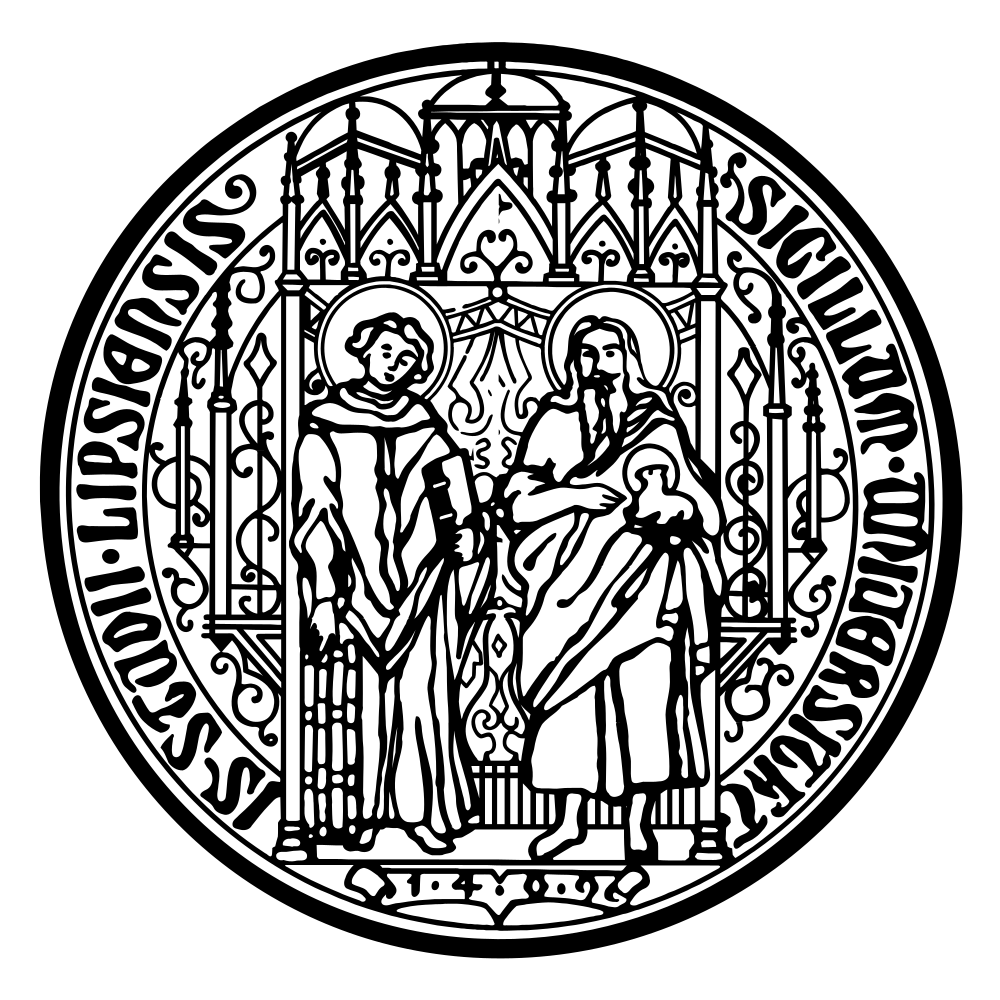
\includegraphics[width=6cm]{Images/UniLeipzig} \\ \medskip % Picture

\mySubtitle \\ \medskip % Thesis subtitle
%\myDegree \\
\myDepartment \\
%\myFaculty \\
\myUni \\ \bigskip

% \myTime\ -- \myVersion % Time and version
\myTime\ 

\vfill

\end{center}
\end{addmargin}

\end{titlepage} % Main title page

% Back of the title page

\thispagestyle{empty}

\hfill

\vfill

\noindent\myName: \textit{\myTitle,} \mySubtitle, %\myDegree, 
\textcopyright\ \myTime

% You may wish to do something with the back of the title page, such as including your supervisors, location or time frame of the work. Below is an example of doing so although you may want to tweak it to your liking.

%\bigskip

%\noindent\spacedlowsmallcaps{Supervisors}: \\
%\myProf \\
%\myOtherProf \\ 
%\mySupervisor

%\medskip \\

%\noindent\spacedlowsmallcaps{Location}: \\
%\myLocation

%\medskip \\

%\noindent\spacedlowsmallcaps{Time Frame}: \\
%\myTime
 % Back of the title page


\cleardoublepage% Abstract

\pdfbookmark[1]{Abstract}{Abstract} % Bookmark name visible in a PDF viewer

\begingroup
\let\clearpage\relax
\let\cleardoublepage\relax
\let\cleardoublepage\relax

\chapter*{Abstract}

The current state of percolation theory is hard to assess. Research often uses different methods, language and notation, is hard to reproduce, and sometimes even provides conflicting results. We aim to give a numerically precise, reproducible overview of the classic 2D percolation problem, along with data and open source code that allow the reader to easily reproduce the results presented, as well as present a simple numerical analysis of the relatively uncommon model called Mandelbrot percolation. We hope to facilitate further research, as well as provide a starting point for anyone interested in the topic.

\endgroup			

\vfill % Abstract page

% \cleardoublepage% Acknowledgements

\pdfbookmark[1]{Acknowledgements}{Acknowledgements} % Bookmark name visible in a PDF viewer

\begin{flushright}{\slshape    
We have seen that computer programming is an art, \\ 
because it applies accumulated knowledge to the world, \\ 
because it requires skill and ingenuity, and especially \\
because it produces objects of beauty.} \\ \medskip
--- \defcitealias{knuth:1974}{Donald E. Knuth}\citetalias{knuth:1974} \citep{knuth:1974}
\end{flushright}

\bigskip

%----------------------------------------------------------------------------------------

\begingroup

\let\clearpage\relax
\let\cleardoublepage\relax
\let\cleardoublepage\relax

\chapter*{Acknowledgements}

% \noindent Put your acknowledgements here.\\

\endgroup % Acknowledgements page

\pagestyle{scrheadings} % Show chapter titles as headings

\cleardoublepage% Table of Contents - List of Tables/Figures/Listings and Acronyms

\refstepcounter{dummy}

\pdfbookmark[1]{\contentsname}{tableofcontents} % Bookmark name visible in a PDF viewer

\setcounter{tocdepth}{2} % Depth of sections to include in the table of contents - currently up to subsections

\setcounter{secnumdepth}{3} % Depth of sections to number in the text itself - currently up to subsubsections

\manualmark
\markboth{\spacedlowsmallcaps{\contentsname}}{\spacedlowsmallcaps{\contentsname}}
\tableofcontents 
\automark[section]{chapter}
\renewcommand{\chaptermark}[1]{\markboth{\spacedlowsmallcaps{#1}}{\spacedlowsmallcaps{#1}}}
\renewcommand{\sectionmark}[1]{\markright{\thesection\enspace\spacedlowsmallcaps{#1}}}

\clearpage

\begingroup 
\let\clearpage\relax
\let\cleardoublepage\relax
\let\cleardoublepage\relax

%----------------------------------------------------------------------------------------
%	List of Figures
%----------------------------------------------------------------------------------------

\refstepcounter{dummy}
%\addcontentsline{toc}{chapter}{\listfigurename} % Uncomment if you would like the list of figures to appear in the table of contents
\pdfbookmark[1]{\listfigurename}{lof} % Bookmark name visible in a PDF viewer

\listoffigures

\vspace{8ex}
\newpage

%----------------------------------------------------------------------------------------
%	List of Tables
%----------------------------------------------------------------------------------------

\refstepcounter{dummy}
%\addcontentsline{toc}{chapter}{\listtablename} % Uncomment if you would like the list of tables to appear in the table of contents
\pdfbookmark[1]{\listtablename}{lot} % Bookmark name visible in a PDF viewer

\listoftables
        
\vspace{8ex}
\newpage
    
%----------------------------------------------------------------------------------------
%	List of Listings
%---------------------------------------------------------------------------------------- 

\refstepcounter{dummy}
%\addcontentsline{toc}{chapter}{\lstlistlistingname} % Uncomment if you would like the list of listings to appear in the table of contents
\pdfbookmark[1]{\lstlistlistingname}{lol} % Bookmark name visible in a PDF viewer

\lstlistoflistings 

\vspace{8ex}
\newpage
       
%----------------------------------------------------------------------------------------
%	Acronyms
%----------------------------------------------------------------------------------------

\refstepcounter{dummy}
%\addcontentsline{toc}{chapter}{Acronyms} % Uncomment if you would like the acronyms to appear in the table of contents
\pdfbookmark[1]{Acronyms}{acronyms} % Bookmark name visible in a PDF viewer

\markboth{\spacedlowsmallcaps{Acronyms}}{\spacedlowsmallcaps{Acronyms}}

\chapter*{Acronyms}

\begin{acronym}[UML]
\acro{DRY}{Don't Repeat Yourself}
\end{acronym}  
                   
\endgroup % Contents, list of figures/tables/listings and acronyms

\cleardoublepage

\pagenumbering{arabic} % Arabic page numbering for thesis content (1, 2, 3, etc)
%\setcounter{page}{90} % Uncomment to manually start the page counter at an arbitrary value (for example if you wish to count the pre-content pages in the page count)

\cleardoublepage % Avoids problems with pdfbookmark

%----------------------------------------------------------------------------------------
%	THESIS CONTENT - CHAPTERS
%----------------------------------------------------------------------------------------


\part{Classic 2D percolation} % First part of the thesis

% Chapter 1

\chapter{Classic percolation}

\label{ch:classicpercolation} % For referencing the chapter elsewhere, use \autoref{ch:introduction} 

%----------------------------------------------------------------------------------------

%----------------------------------------------------------------------------------------

\section{1D Case: toy model}\label{sec:1d}

\subsection{Percolation threshold $p_c$}

\subsection{Critical exponent $\sigma$}

\subsection{Critical exponent $\gamma$}

\subsection{Critical exponent $\nu$}


%----------------------------------------------------------------------------------------

\section{2D case in square lattice}\label{sec:2dsquare}


\subsection{Critical exponents}

\subsection{Correlation length}

\subsection{Phase transitions}

\subsection{Real space renormalisation}


%----------------------------------------------------------------------------------------

\section{Bethe lattice}\label{sec:2dgeneral}




 
\afterpage{\blankpage}
\chapter{Classical percolation - experimental methods and results} 
\label{ch:classical_experimental}


%----------------------------------------------------------------------------------------

%----------------------------------------------------------------------------------------

To experimentally verify the results described above, we ran more than \textbf{3 billion simulations}, generating approximately \textbf{250GB} of data. The code that used to run the simulation and to extract the statistics is available on Github, see \autoref{chap:code} for more details. The full data is also available, see \autoref{chap:data}. 


\section{2D lattice simulation}
\label{sec:2d_lattice_simulation}


We used a $L \times L$ square, periodic lattice, which is topologically equivalent to a torus. Each node has four neighbours: one above it, one to the right, one below, and one to the left. The periodicity is represented by the fact that the right neighbors of the nodes in the rightmost column are the nodes in the leftmost column. Similarly, the left neighbours of the leftmost column are the nodes in the rightmost column, the top neighbours of the topmost row are the nodes in the bottom-most row, and the bottom neighbours of the bottom-most row are nodes in the topmost row.

Each node can be in one of two states: dead or alive. Initially, all nodes are in the alive state. With probability $p$, we change state of each individual node to dead. We then compute and store the set of clusters found in the lattice. A cluster is a set of connected nodes sharing the same state. 

Each cluster can either be a finite or infinite. Since the lattice is periodic, \textbf{a cluster is considered infinite if its 1D extension in either direction is greater than or equal to the size of the lattice $L$}. Otherwise, it is a finite cluster. In other words, we imagine a bounding box around each cluster, and if at least of the dimensions of the box is greater than or equal to $L$, the cluster is infinite. 

We generated around 3000 lattices for each pair $(p, L)$, with $p$ ranging from 0 to 1 (with a higher density near the critical points) and $L$ ranging from 16 to 1024.


\section{Percolation probability}
\label{sec:sim_perc_prob}

A lattice has percolated if it contains at least one infinite cluster. For each $(p, L)$, we count the number of percolating lattices and divide by the total number of lattices simulated to compute the percolation probability.

In \autoref{fig:sim_perc_prob_1}, we plot the percolation probability against the occupation probability $p$ for various lattice sizes.


\begin{figure}[H]
  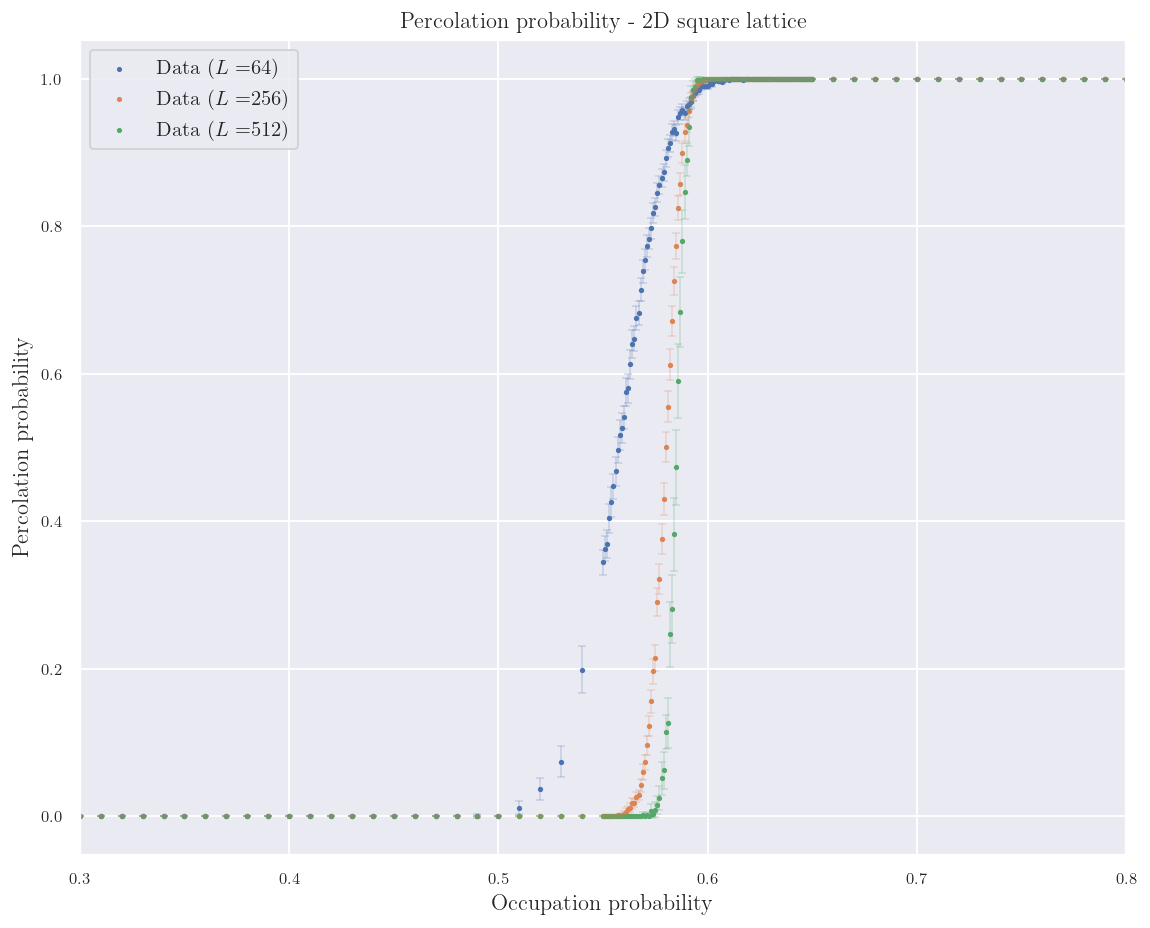
\includegraphics[width=\linewidth]{Images/sim_perc_prob_1.png}
  \caption{Percolation probability curve for various lattice sizes}
  \label{fig:sim_perc_prob_1}
\end{figure}

By visual inspection, we can hypothesize that the curve is a hyperbolic tangent curve: 

$$ 
y(x) = \tanh(x)
$$

We can shift and scale this function so that it's centered at $x=\beta$, and such that it's domain matches our data, i.e. $\mathcal{D}(y) = \left[ 0, 1 \right]$. We'd also like a parameter that controls how steep the transition is between $y=0$ and $y=1$ - this can be done by scaling $x$ by a multiplicative factor $\alpha$. The function becomes

$$ 
y(x) = \frac{\tanh(\alpha(x - \beta)) + 1}{2}
$$ 

In \autoref{fig:sim_perc_prob_2}, we can see the the fitted data points. \autoref{table:sec3_tahn_fit_parameters} contains the precise values.


\begin{figure}[H]
  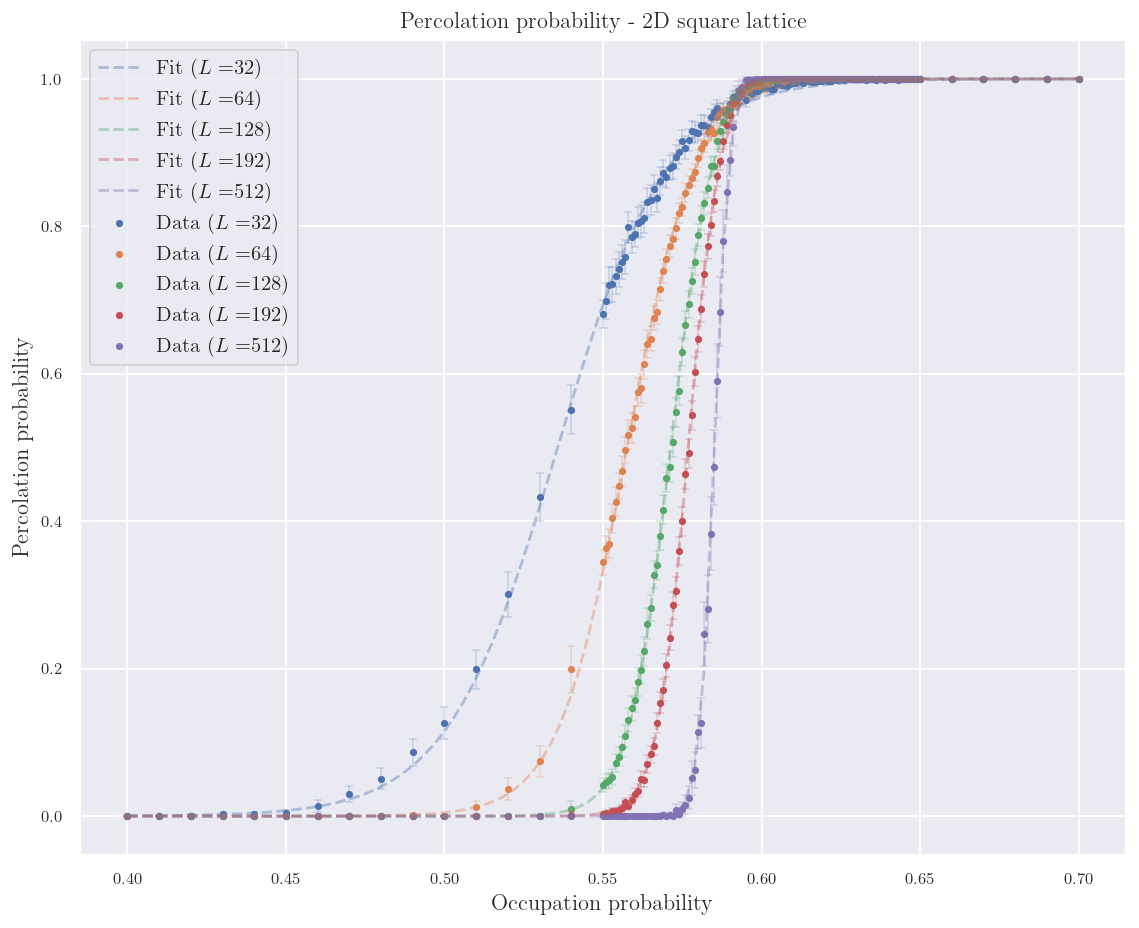
\includegraphics[width=\linewidth]{Images/sim_perc_prob_2.png}
  \caption{Percolation probability with a hyperbolic tangent LMS fit}
  \label{fig:sim_perc_prob_2}
\end{figure}

We notice that the the bigger the lattice, the faster it jumps from $y=0$ to $y=1$. This is consistent with the widely known fact that as L increases, i.e. in the limit $L \rightarrow \infty $, the transition becomes a step function at $p = p_c$. 

Another interesting fact to notice is that with the structure of the function we're fitting, $\beta$ represents the point at which the percolation probability first reaches $\frac{1}{2}$.

These two observations suggest that studying the behaviour of $\alpha$ and $\beta$ as a function of the lattice size $L$ might be interesting. We can see the results obtained in \autoref{fig:sim_perc_prob_param_scaling.png}, in a so called finite-size scaling analysis.

\begin{figure}[H]
  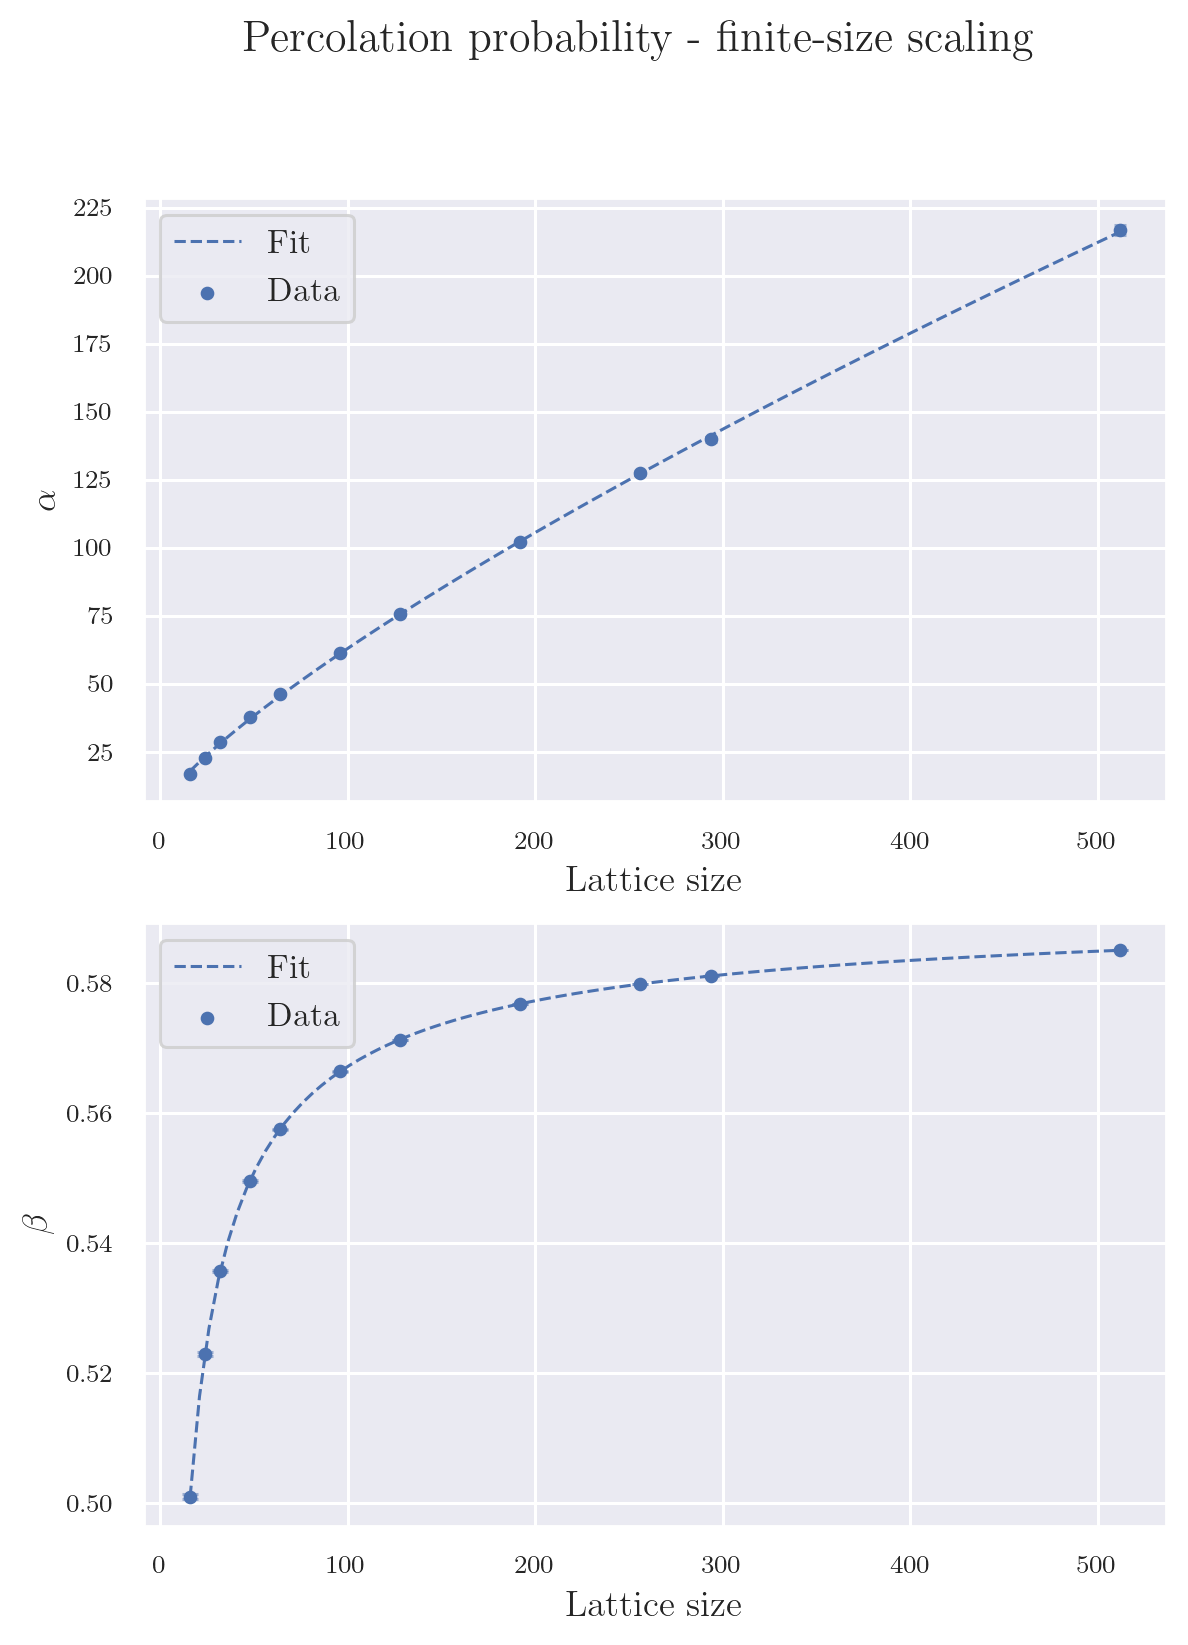
\includegraphics[width=\linewidth]{Images/sim_perc_prob_param_scaling.png}
  \caption{Finite-size scaling analysis of the hyperbolic tangent function}
  \label{fig:sim_perc_prob_param_scaling.png}
\end{figure}

We observe a monotonic growth in $\alpha$ as a function of the lattice size $L$. We were able to get a reasonable fit by using the ansatz

$$ 
    \alpha(L) = a L^n + b
$$

The precise values for the constants $a$, $n$ an $b$ can be seen in \autoref{table:pp_slope_finite_size_scaling_params}.

Of course, 
$$ 
\lim_{L\to\infty} a L^n + b = \infty \hspace{0.5cm} a > 0, n>0
$$

Since $\alpha$ controls how steep the hyperbolic tangent curve is, that is, how fast it goes from 0 to 1, this supports the hypothesis that as we increase $L$, the curve gets arbitrarily close to a step function. 


The parameter $\beta$, on the other hand, behaves differently. We were able to get a fairly good fit by using the ansatz 

$$ 
\beta(L) = c - a e^{-\frac{L^n}{b}}
$$ 

The precise values for $a$, $n$, $b$ an $c$ can be seen in \autoref{table:pp_center_finite_size_scaling_params}. 

It is clear that 
$$ 
\lim_{L\to\infty} c - a e^{-\frac{L^n}{b}} = c
$$

Since $\beta$ represents occupation probability at which the percolation probability reaches 1/2, the limit above allows us to estimate $p_c$, the critical probability of our system - we do so by interpreting $p_c$ as $\beta$ in the limit of an infinite lattice. This value comes out to be $\mathbf{0.5907} \pm 0.006$.
The error estimates for the percolation probability were computed by treating it as a Bernoulli random variable. We used a 99\% confidence interval and the expression 

$$ 
\textrm{Error} = z \sqrt{\frac{\bar{p}(1-\bar{p})}{n}}
$$

where z is the value coming from the z-table for the desired confidence interval (numerically, $z=2.576$), $\bar{p}$ is the mean of the observations, and $n$ is the number of observations\cite{bertsekas2008introduction}.

\section{Percolating cluster strength}
\label{sec:sim_perc_clust_strength}

The percolating cluster strength represents the probability that a randomly picked node belongs to a infinite cluster. This was numerically approximated by counting the number of nodes belonging to the (possibly multiple) infinite clusters and dividing by the total number of nodes. The results obtained can be seen in \autoref{fig:sim_perc_clust_strength_1}.

\begin{figure}[H]
  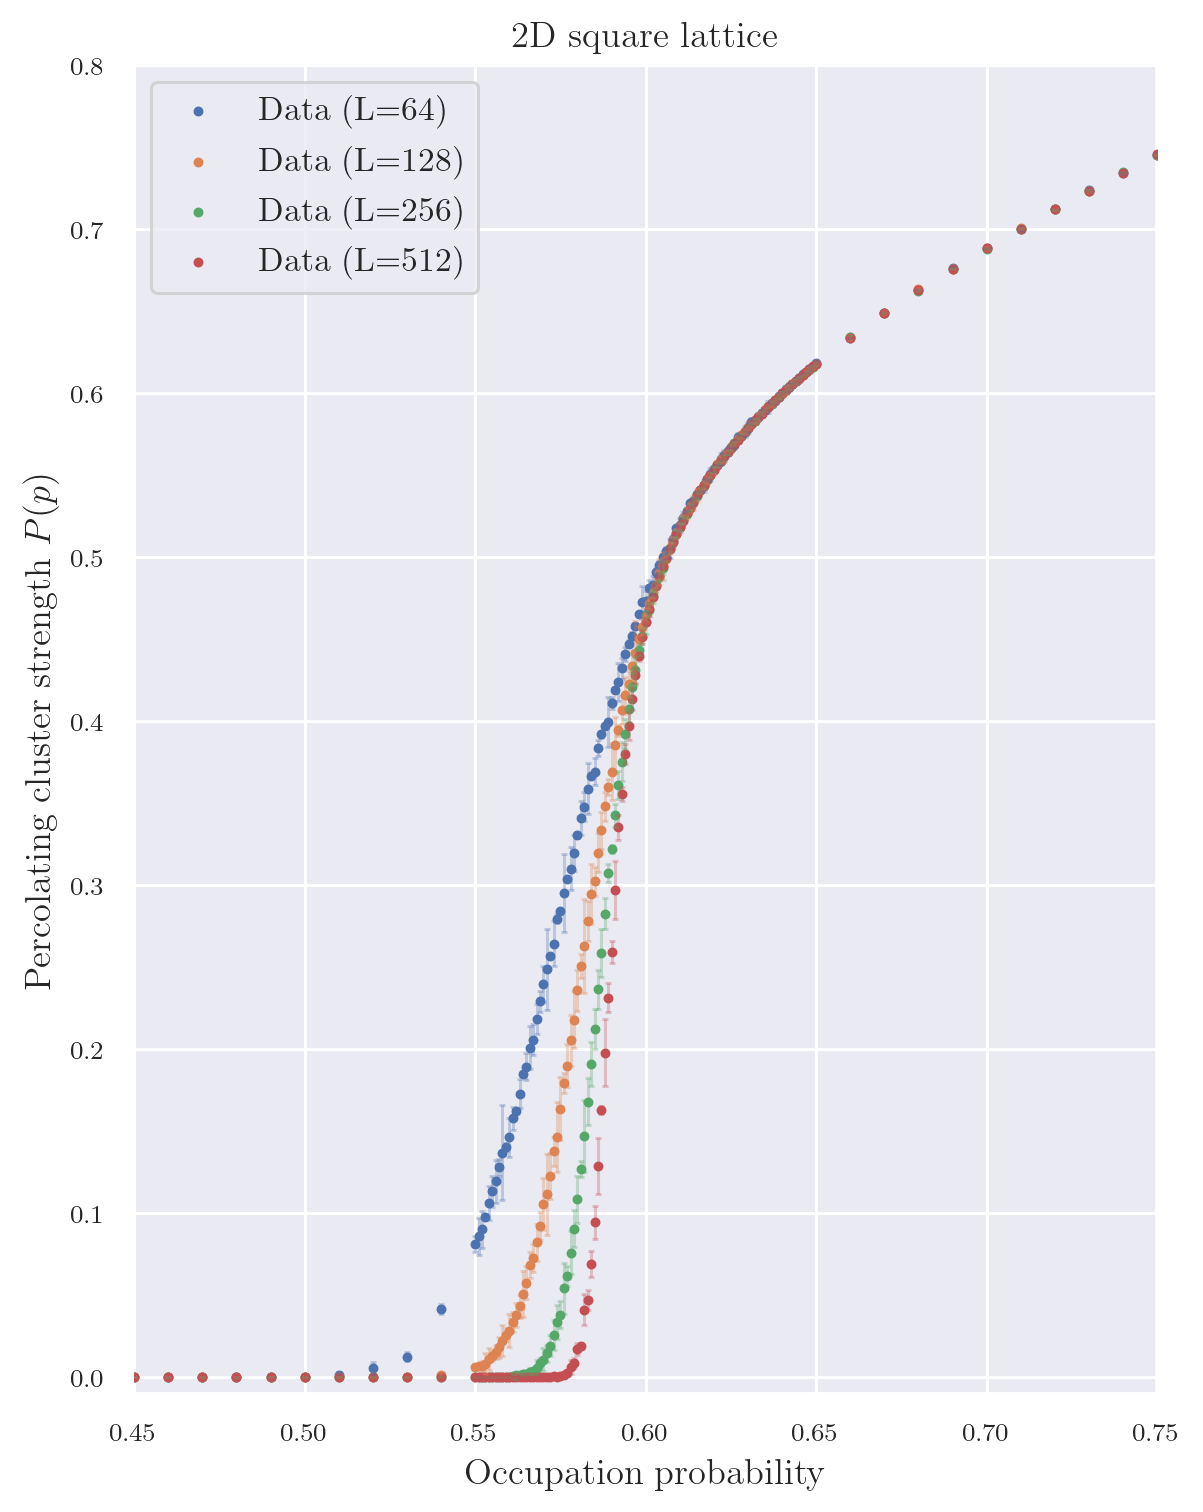
\includegraphics[width=\linewidth]{Images/sim_perc_clust_strength_1.png}
  \caption{Percolating cluster strength versus occupation probability for various lattice sizes.}
  \label{fig:sim_perc_clust_strength_1}
\end{figure}

As discussed in \autoref{sec:th_percolating_cluster_strength}, we expect to see the percolating cluster strength $P(p)$ go from being zero for $p < p_c$ to a non-zero value for $p > p_c$. This is precisely what we see in \autoref{fig:sim_perc_clust_strength_1}. It's also possible to notice that the transition becomes more abrupt for larger lattice sizes, which provides evidence for intuition that this transition approaches a step function as $L \to \infty$.
Unfortunately, we were not able to find an ansatz that approximates this curve well, and therefore can't provide at this time a convincing numerical estimation for the "abruptness" of this transition or how fast it approaches the step function. 





The errors in the calculation of $P(p)$ were estimated by splitting all observations for each $p$ (around 2000) into 20 bins, computing the mean value for $P(p)$ in each bin, and then computing the standard deviation mean values obtained across the different bins.


\section{Mean cluster size}
\label{sec:sim_mean_clust_size}

The mean cluster size $\chi(p)$ represents the average number of nodes in the finite clusters as defined in \autoref{sec:2d_lattice_simulation}. For each simulation, we loop over the finite clusters, adding their sizes. We then divide the sum by the number of finite clusters to get the average in a particular simulation/lattice. Afterwards, we average again, this time over lattices (of course, this averaging is only done over lattices with the same occupation probability $p$ and size $L$). 


The results can be seen in \autoref{fig:sim_mean_cluster_size_1}.



\begin{figure}[H]
  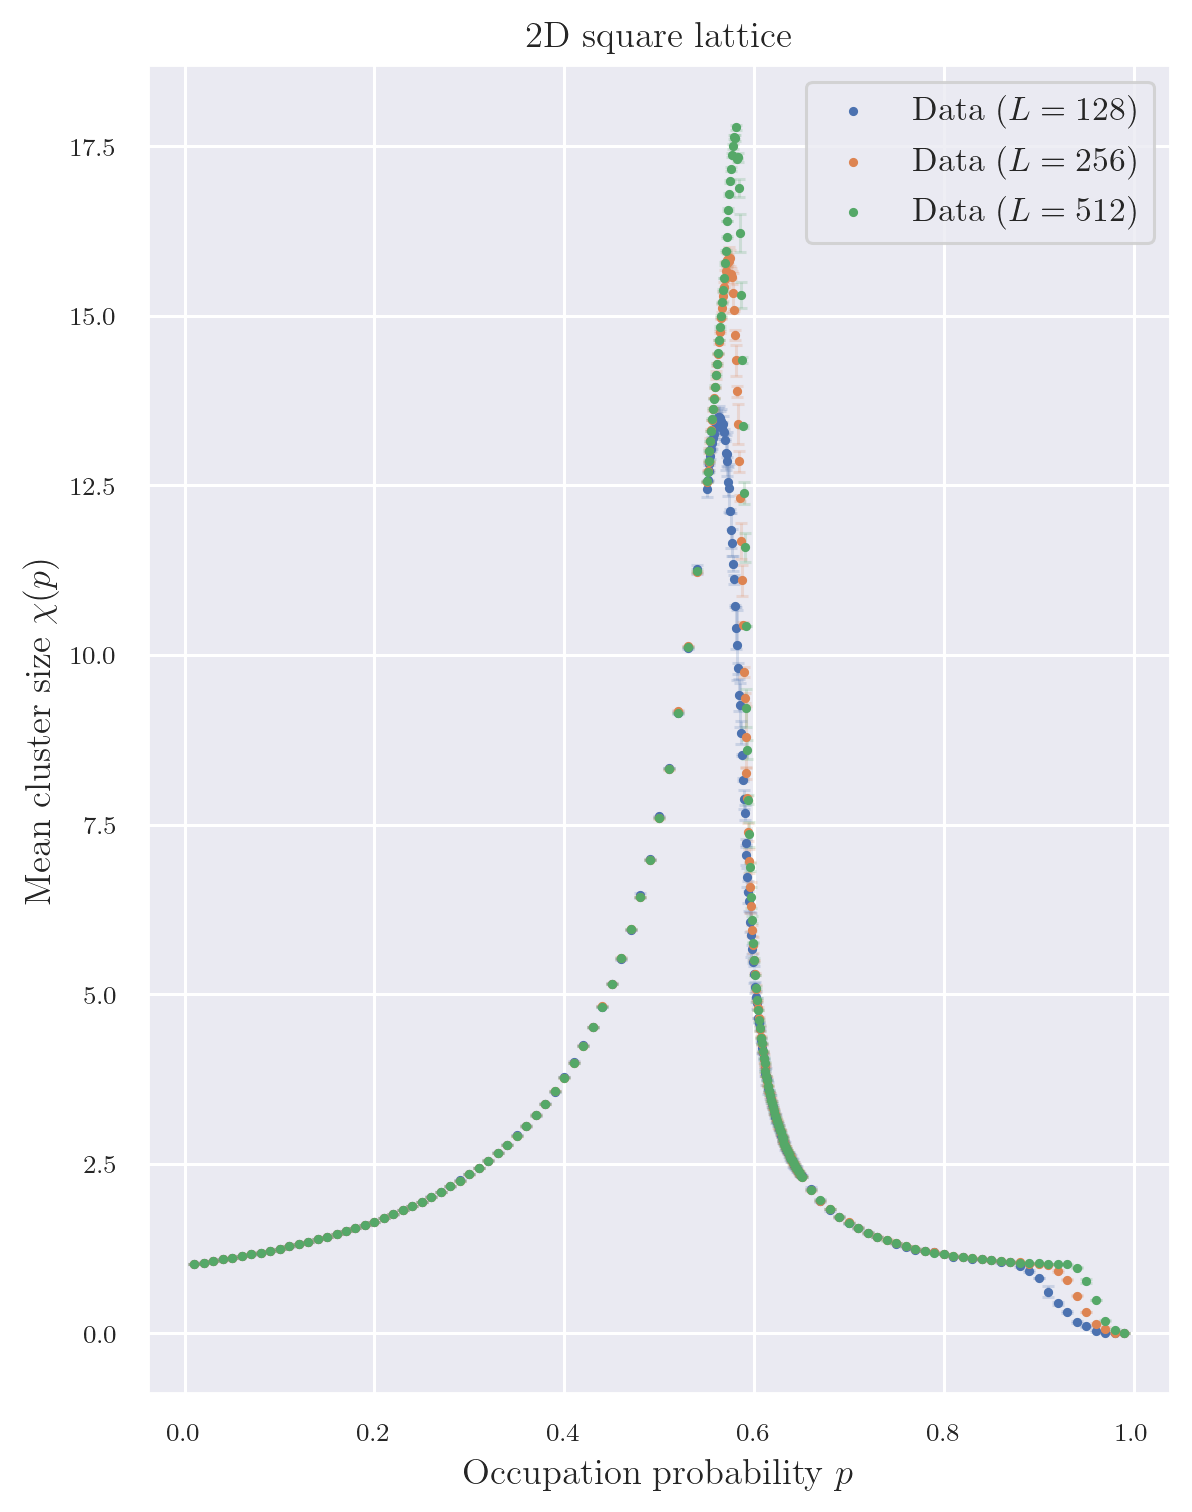
\includegraphics[width=\linewidth]{Images/sim_mean_cluster_size_1.png}
  \caption{Mean finite cluster size versus occupation probability for various lattice sizes}
  \label{fig:sim_mean_cluster_size_1}
\end{figure}


As expected, we see a monotonic increase in $\chi(p)$ up to a maximum value, corresponding to some sort of critical value, and then a somewhat faster, monotonic decrease after the maximum. There is also an interesting kink close to $p=0.9$ which we did not investigate further.
The presence of this peak immediately presents itself as an opportunity to check some of the ideas and scaling laws presented in \autoref{sec:th_mean_cluster_size}. 


As a starting point, we study the peak position and height for each lattice size. Our goal is to make an educated guess on how these values change as we increase the lattice size. To estimate the peak height and occupation probability (the peak position), we fitted a parabola to the 10 points closest the numerical peak (the point for which the height is maximum).

\autoref{fig:sim_mean_cluster_size_peak_height} shows the peak height $H$ as a function of the lattice size we obtained from our data, and \autoref{table:pp_mean_cluster_size_peak_values} shows the precise values obtained.

\begin{figure}[H]
  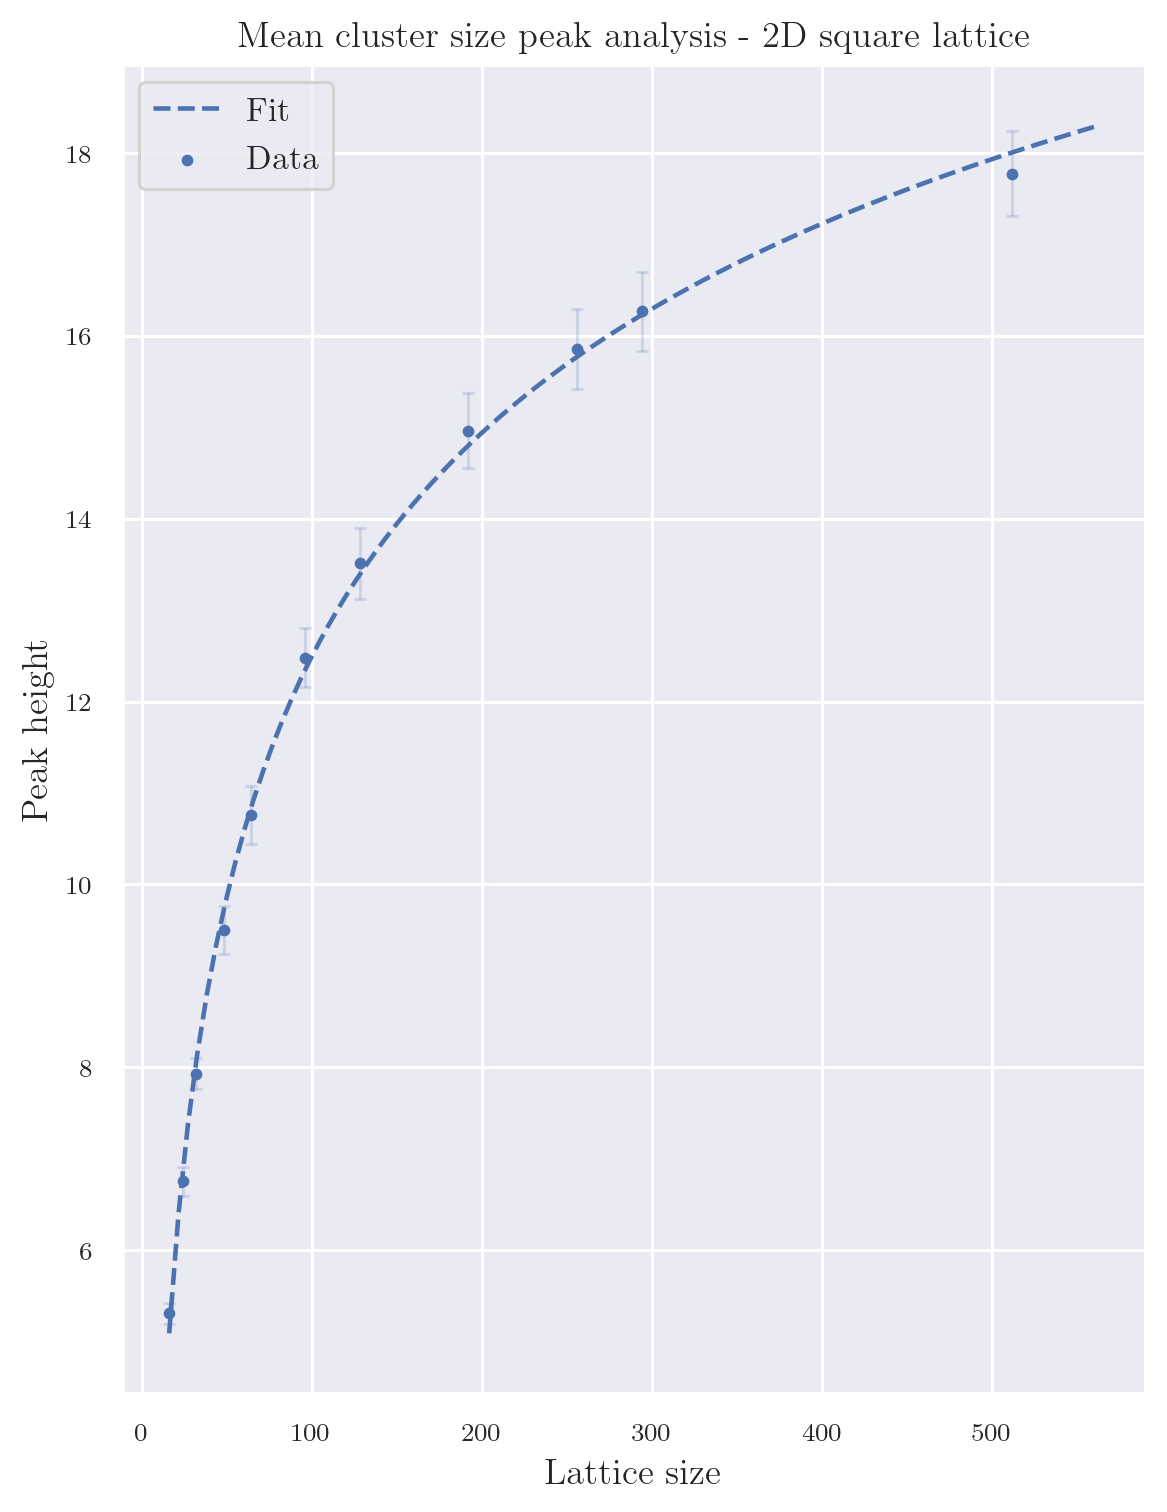
\includegraphics[width=\linewidth]{Images/sim_mean_cluster_size_peak_height.png}
  \caption{Mean cluster size, peak height for various lattice sizes}
  \label{fig:sim_mean_cluster_size_peak_height}
\end{figure}

As expected, the height grows with the lattice size. The ansatz used to fit the curve is
$$ 
H(L) = a \log(bL)^c + d
$$

The precise values of $a$, $b$, $c$ and $d$ can be seen in \autoref{table:pp_mean_cluster_size_peak_height_finite_size_scaling_params}. Even thought some of the numerical values obtained from the least squares fit show somewhat high variance and correlation with other parameters, this on itself does not present a problem for us here, since we're not interested in estimating any parameter in particular.

Since 
$$
\lim_{L\to\infty} a \log(bL)^c = \infty
$$

This data supports the hypothesis that as we increase $L$, the peaks height does not converge to any finite height, and instead diverges.


Next, we consider the peak position $K$ as a function of the lattice size $L$. While the peak height is expected to diverge, as discussed above, one expects that the peak probability would converge the true percolation threshold $p_c$ as $L$ increases. 
\autoref{fig:sim_mean_cluster_size_peak_position} shows the probability at which the peak is located, $K$, as a function of lattice size, and \autoref{table:pp_mean_cluster_size_peak_positions} shows the numerical values.


\begin{figure}[H]
  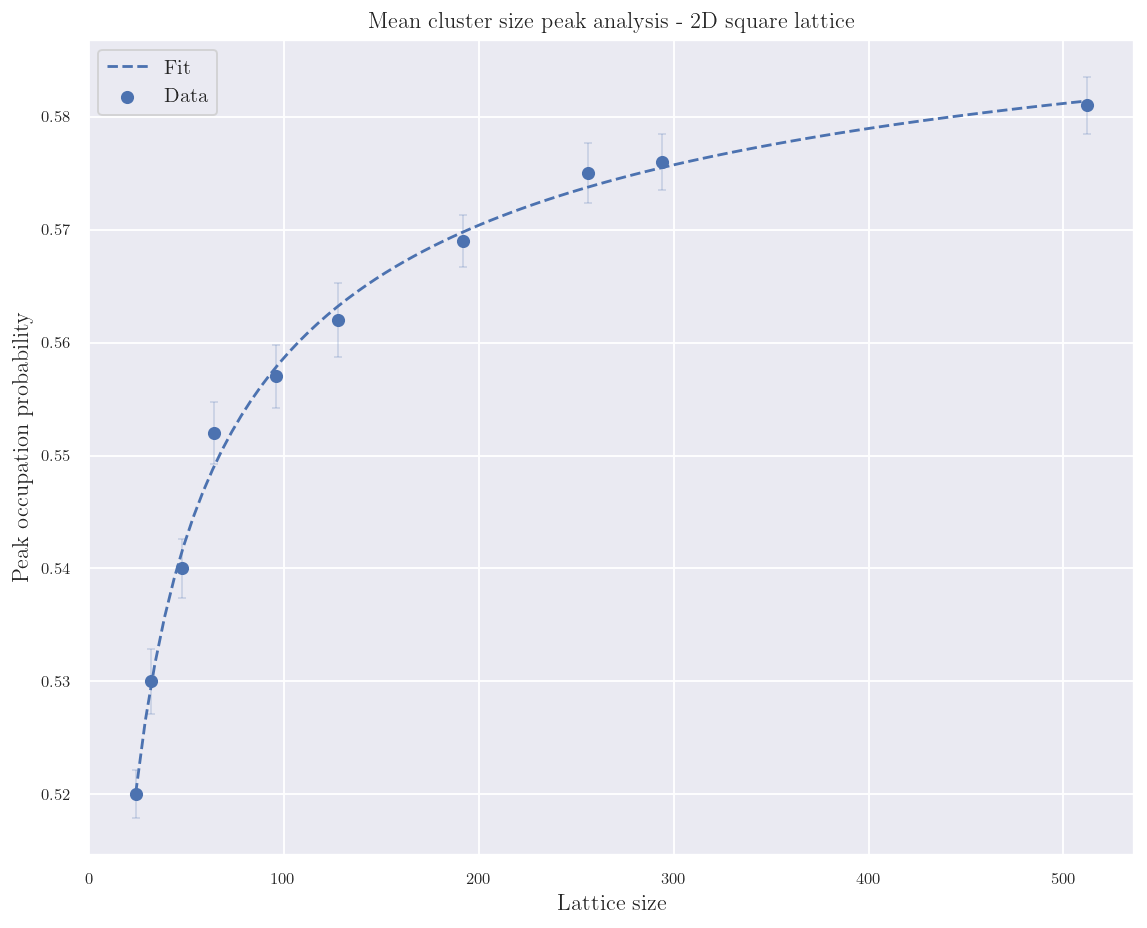
\includegraphics[width=\linewidth]{Images/sim_mean_cluster_size_peak_position.png}
  \caption{Mean cluster size, peak position for various lattice sizes}
  \label{fig:sim_mean_cluster_size_peak_position}
\end{figure}


The ansatz used in the fit above is again

$$ 
    K(L) = c - a e^{\frac{L^n}{b}}
$$

So we conclude that this is, as predicted, evidence for the percolation threshold converging to a finite numerical value (namely, $c$). The precise values for all the fit parameters can be seen in \autoref{table:pp_mean_cluster_size_peak_position_finite_size_scaling_params}. Using this method, we estimate $p_c$ to be \textbf{0.5986} $\pm$ 0.009 (again, it's worth pointing out that even though some of the parameters present a somewhat high variance, the one that we're interested in, i.e. $c$, has a surprisingly low variance and correlation with other parameters, further supporting our hypothesis).

The errors in the calculation of $\xi(p)$ were estimated by splitting all observations for each $p$ (around 2000) into 20 bins, computing the mean value for $P(p)$ in each bin, and then computing the standard deviation mean values obtained across the different bins. For the peak position and height, we errors were computing by taking the square root of the relevant diagonal term in the covariance matrix obtained from the least squares fit.

\section{Correlation function and correlation length}


Lastly, we turn our attention to the study of the correlation length. These are a quantities of great interest in general. Apart from being relevant in the study of many phenomena, they also have an intuitive interpretation: the correlation function, for example, can be used to assess the distance required between nodes for the values to be effectively uncorrelated. This distance is generally called the correlation length.

For each lattice simulation, the correlation function was estimated by  selecting a large number (approximately 200000) of random node pairs from the lattice, computing the distance between the nodes in the pair, and then checking whether they belong to the same finite cluster. Averaging over all selected pair a given distance $r$ away, this gives us an estimate of the probability of nodes whose distance is $r$ belonging to the same finite cluster, which is the definition of the correlation function $g(r)$. We then average this over many lattices.

To estimate the correlation length $\xi$, we use the fact that
$$ 
 g(r) \propto r^{-\nu} e^{-\frac{r}{\xi}}
$$ 

Which covers both the case in which $p=p_c$, and the case in which $|p - p_c| \ll 1$. It is somewhat surprising that this also provides a good approximation for the correlation function when even $|p - p_c| > 1$.


The results for the correlation function can be seen in \autoref{fig:sim_corr_func_1}, along with the best fit using the ansatz above. Notice that this plot uses a logarithmic scale in the vertical direction. We give a higher weight to points with bigger $r$ - the reason for this is that the approximation gets better the bigger $r$ is (our goal is to approximate $\xi$, and its influence is only relevant for larger values of $r$). So even though the fit is not great for smaller values of $r$, this allows us to see the exponential decay, represented by the fact that the points are fitted to a line, fairly well.


One interesting fact to mention here is that we get much better results if we use the Manhattan distance, as opposed to the Euclidean distance. The reason for this is not completely clear, but we hypothesize that this is because the Manhattan distance better matches the geometry of the lattice - a "diagonal neighbour", for example, is really two time further away than a nearest neighbour, as opposed to $\sqrt{2}$ times further away, which is what the Euclidean distance would give us.

\autoref{fig:sim_corr_length_1} shows the correlation lengths obtained for multiple lattice sizes and occupation probabilities. 


\begin{figure}[H]
  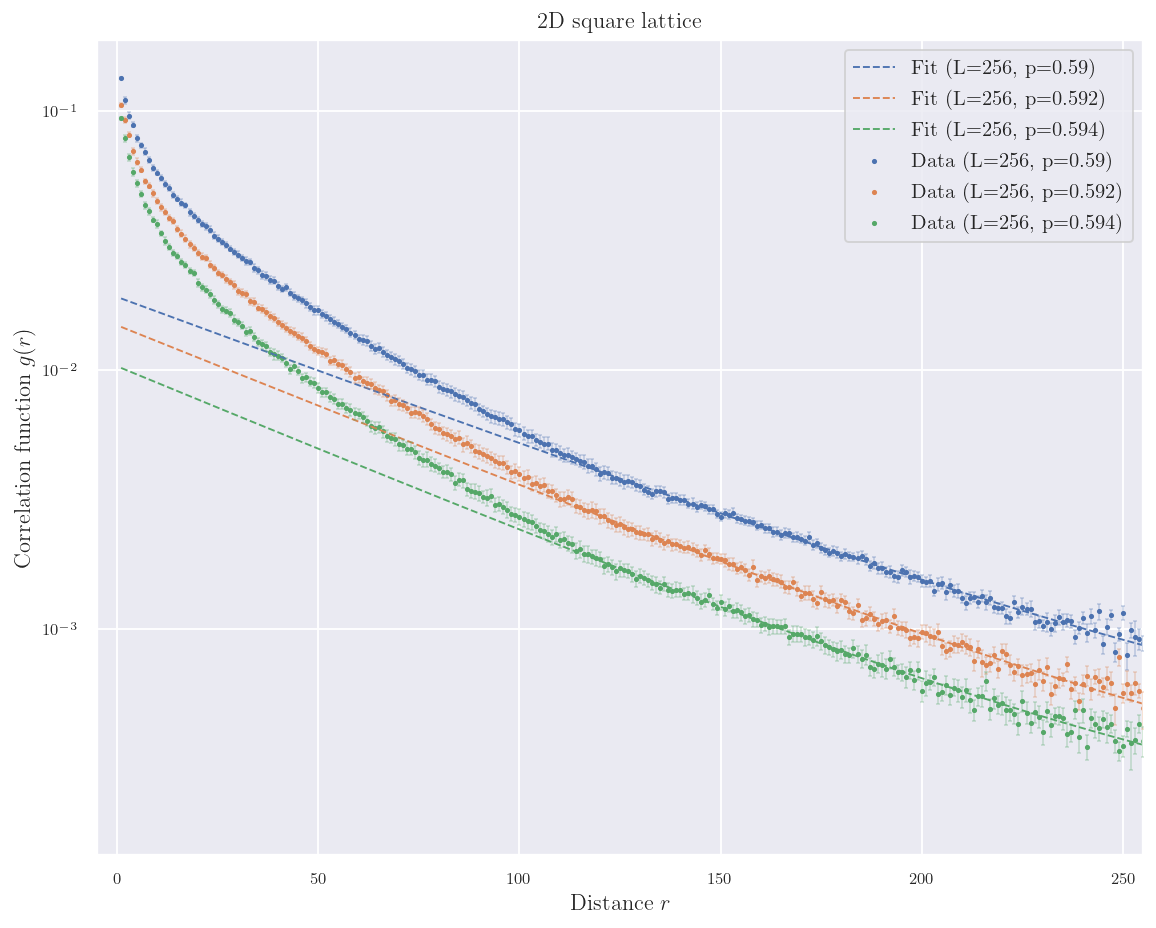
\includegraphics[width=\linewidth]{Images/sim_corr_func_2.png}
  \caption{Correlation function for various sizes and occupation probabilities logarithmic scale in the vertical direction)}
  \label{fig:sim_corr_func_1}
\end{figure}

There's a couple of interesting things to notice in \autoref{fig:sim_corr_length_1}. 
The first is that errors are greatly increased to the right of the peaks. This happens because the errors in the correlation function increase when the occupation probability is in that range - and that, in turn, happens because as we increase the occupation probability $p$ past the $p_c$, many smaller merge clusters merge into the infinite cluster. So it gets much harder to find two pairs of nodes that are not part of the infinite cluster - essentially causing to correlation function to become closer and closer to being identically zero.

More interestingly, though, is to compare the numerical values for correlation length with the square root of the mean cluster size. The square root is necessary since the mean cluster size is closer to an area, since it gives us the average number of nodes in a cluster. By taking its square root, we obtain some kind of "average linear size". By comparing this with the correlation length, we can see that the difference is bigger closer to the peaks, indicating finite size artifacts start to appear. Farther from the peak (which is also roughly the critical occupation probability), these two values are close to each other, indicating that the size of the lattice is sufficiently large so as to be representative of an infinite lattice. 


\begin{figure}[H]
  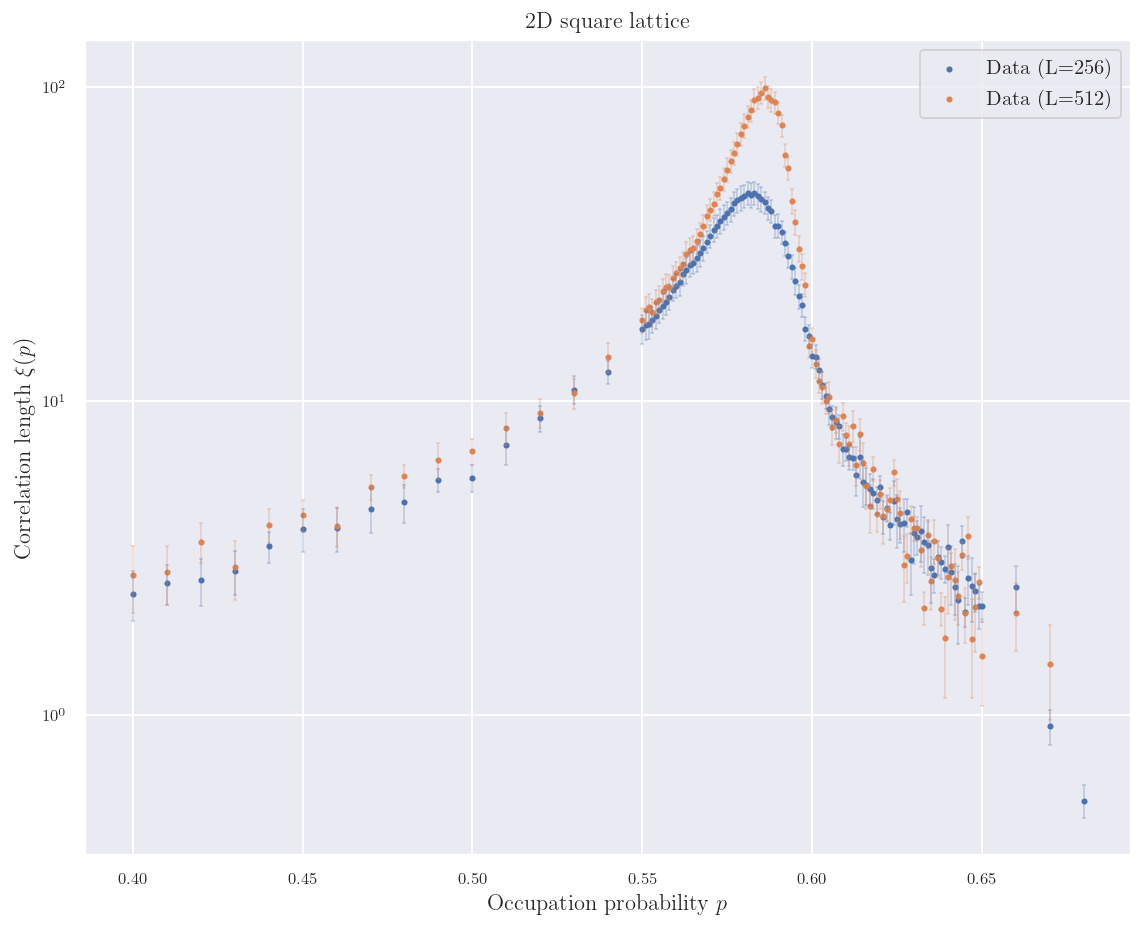
\includegraphics[width=\linewidth]{Images/sim_corr_length_1.png}
  \caption{Correlation length for multiple lattice sizes (logarithmic scale in the vertical direction)}
  \label{fig:sim_corr_length_1}
\end{figure}
    

With this, we finish our analysis of the classical percolation model. Next, we'll look at the so called Mandelbrot percolation model. 
\afterpage{\blankpage}
\part{Mandelbrot percolation}
\chapter{Mandelbrot percolation - methods and results}
\label{ch:mandelbrot_experimental}

\section{Introduction}

Now we turn our attention to the so called Mandelbrot percolation, which is also known in the literature as Fractal percolation. The idea is, again, to study the clusters structure and distribution, but the coloring of the lattice happens in a different way: instead of doing a single pass over the lattice and coloring the nodes at random, we do this process repeatedly - at each step, we subdivide each node in the lattice into a number of "sub-nodes" and color the remaining "alive" (not yet colored) nodes with probability $p$. An illustration of this process can be seen in \autoref{fig:mandelbrot_process}. 
Each iteration generates a lattice $A_n$ (which is, of course, highly correlated with the previous lattice $A_{n-1}$). Mandelbrot percolation is the study of the limit of this process the number of steps increases arbitrarily, that, is $\lim_{n\to\infty} A_n$.

\begin{figure}[H]
  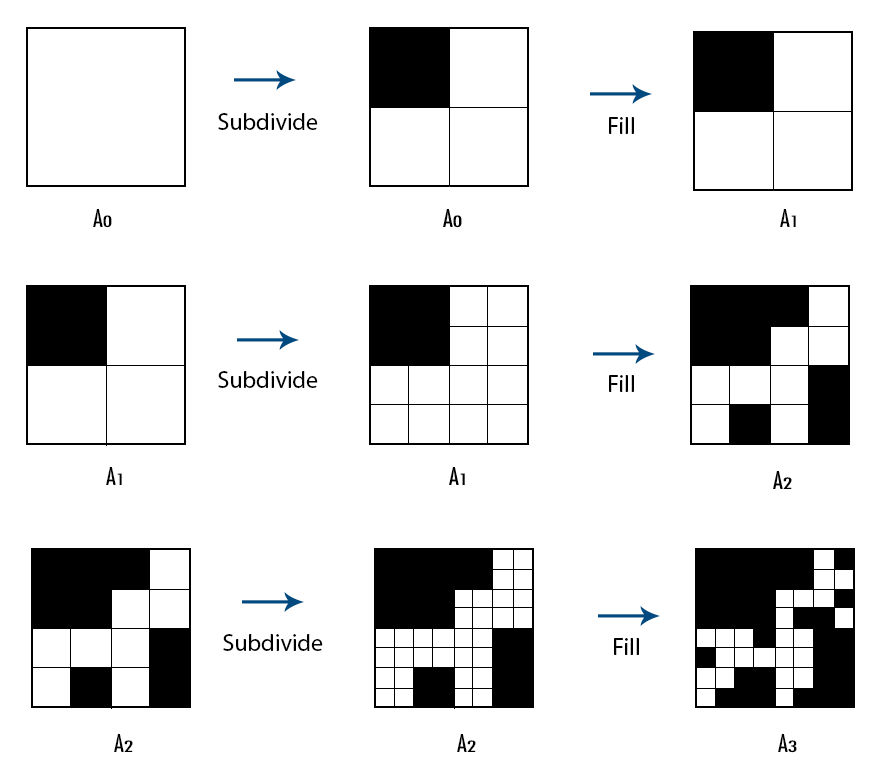
\includegraphics[width=\linewidth]{Images/mandelbrot_process.png}
  \caption{Illustration of the Mandelbrot percolation iteration process, showing three iterations}
  \label{fig:mandelbrot_process}
\end{figure}


\begin{figure}[H]
  \includegraphics[width=\linewidth]{Images/mandelbrot_lattice.png}
  \caption{A Mandelbrot percolation lattice after 11 iterations}
  \label{fig:mandelbrot_lattice}
\end{figure}


\section{Simulation methods}

The simulations were run, again, on a 2D periodic square lattice. 
We studied three properties: the percolation probability, mean cluster size and percolating cluster strength. We explicitly used exactly the same definitions, methods and algorithms as for the 2D case - the reason for this is that this way, a direct comparison is possible. The precise description of these methods is available in \autoref{ch:classical_experimental}.

\section{Percolation probability}

In \autoref{fig:simm_perc_prob_2}, the first thing we notice is that the the critical probability $p_c$ is much lower than in the classical percolation model - at first sight, it's clear that $p_c < 0.3$. The reason for this is somewhat obvious. For a given $(p, L)$ pair, in classical percolation, we do a single pass over the lattice, whereas in the Mandelbrot model, we have done several passes previously, when the lattice was smaller. So on top of making multiple passes, the previous passes happened when each node represented a bigger part fraction of the lattice.

\begin{figure}[H]
  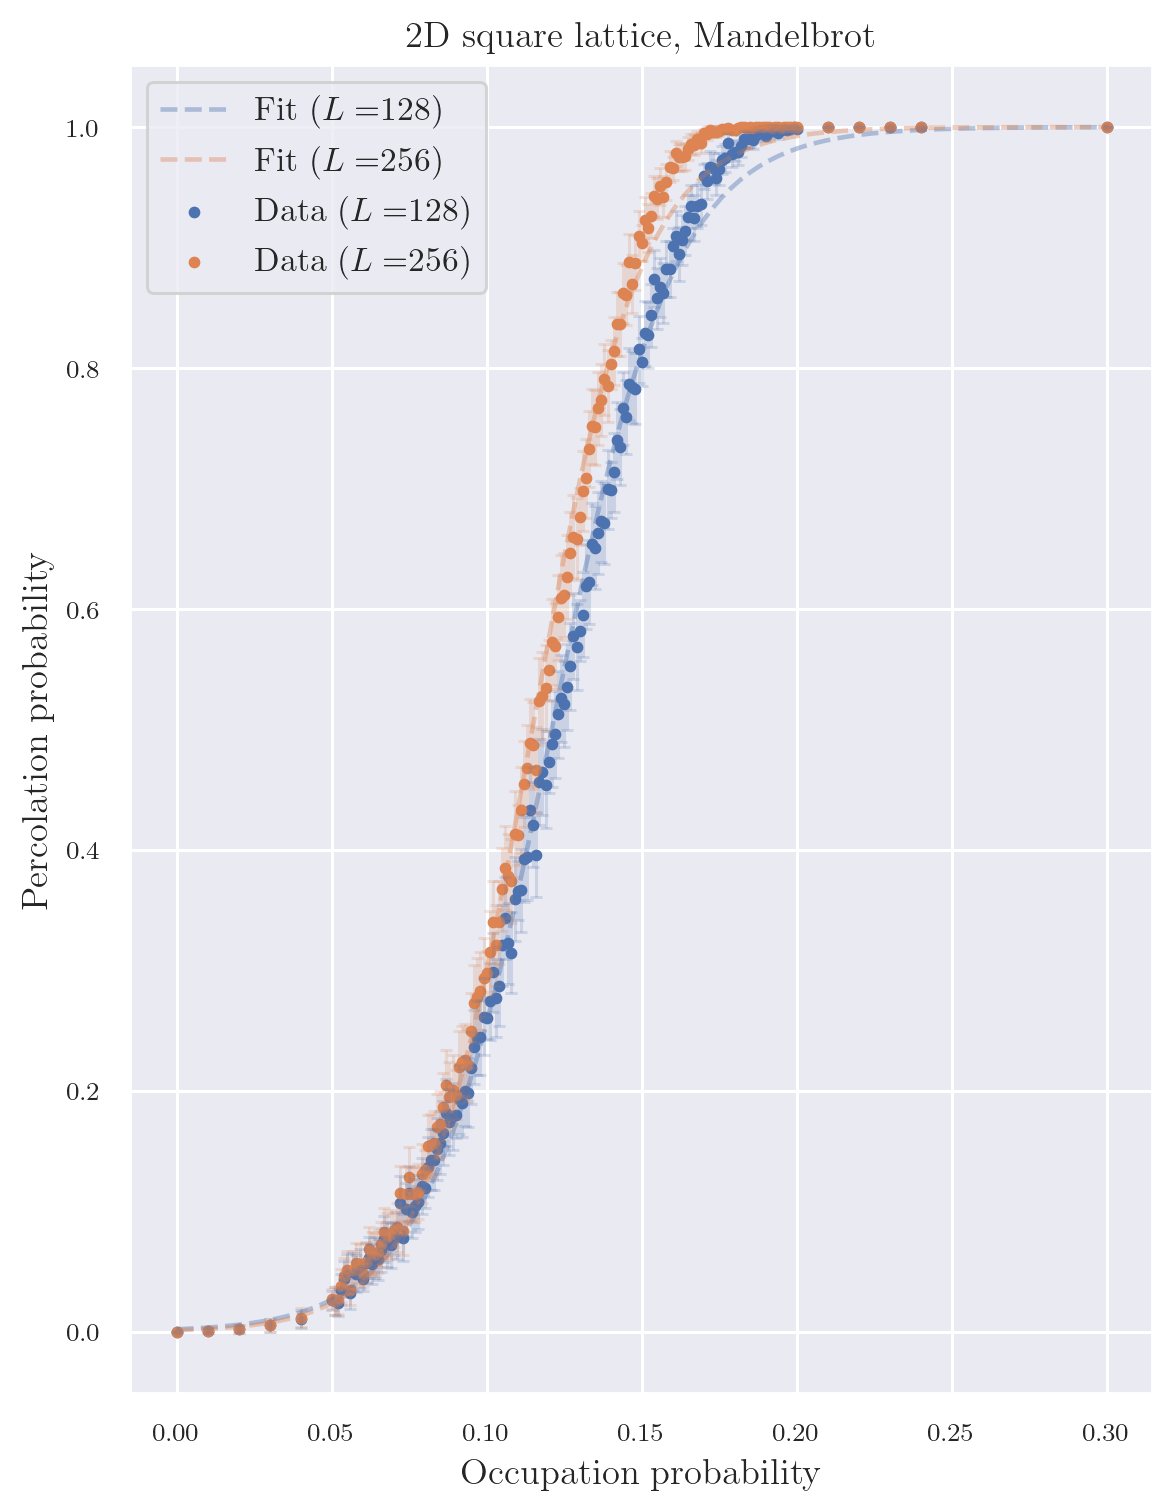
\includegraphics[width=\linewidth]{Images/simm_perc_prob_2.png}
  \caption{Percolation probability in the Mandelbrot percolation model}
  \label{fig:simm_perc_prob_2}
\end{figure}

Just like in classical percolation, we fitted a hyperbolic tangent function to the data, and for $L=256$, which is the largest size we simulated for the Mandelbrot model, we find that the the percolation probability reaches the $0.5$ mark when $p=\textbf{0.1273} \pm 0.021$. We point out that the fit is noticeably worse for the Mandelbrot model than in the case of classical percolation, which suggests an underlying fundamental difference between the models. Additionally, we notice that plots obtained for $L=128$ and $L=256$ are in relation to each other in a different way than the equivalent curves in the classical percolation case. In comparison with \autoref{fig:sim_perc_prob_2}, for example, one notices that whereas there, the curves have a sharp increase at very different occupation probabilities, here they are much closer to each other for low values of $p$, and remain much closer. We hypothesize that this happens, again, because the lattices are much more closely related here - the additional pass used in the $L=256$ happens at a smaller length scale and therefore has a less pronounced effect on the curve.

The errors were computed using the same method as described in \autoref{sec:sim_perc_prob}.

\section{Percolating cluster strength}

The percolation cluster strength results for the Mandelbrot percolation simulations can be seen in \autoref{fig:simm_perc_clust_strength_1}. The curve looks qualitatively pretty similar to the one we had for classical percolation (see \autoref{fig:sim_perc_clust_strength_1}).


\begin{figure}[H]
  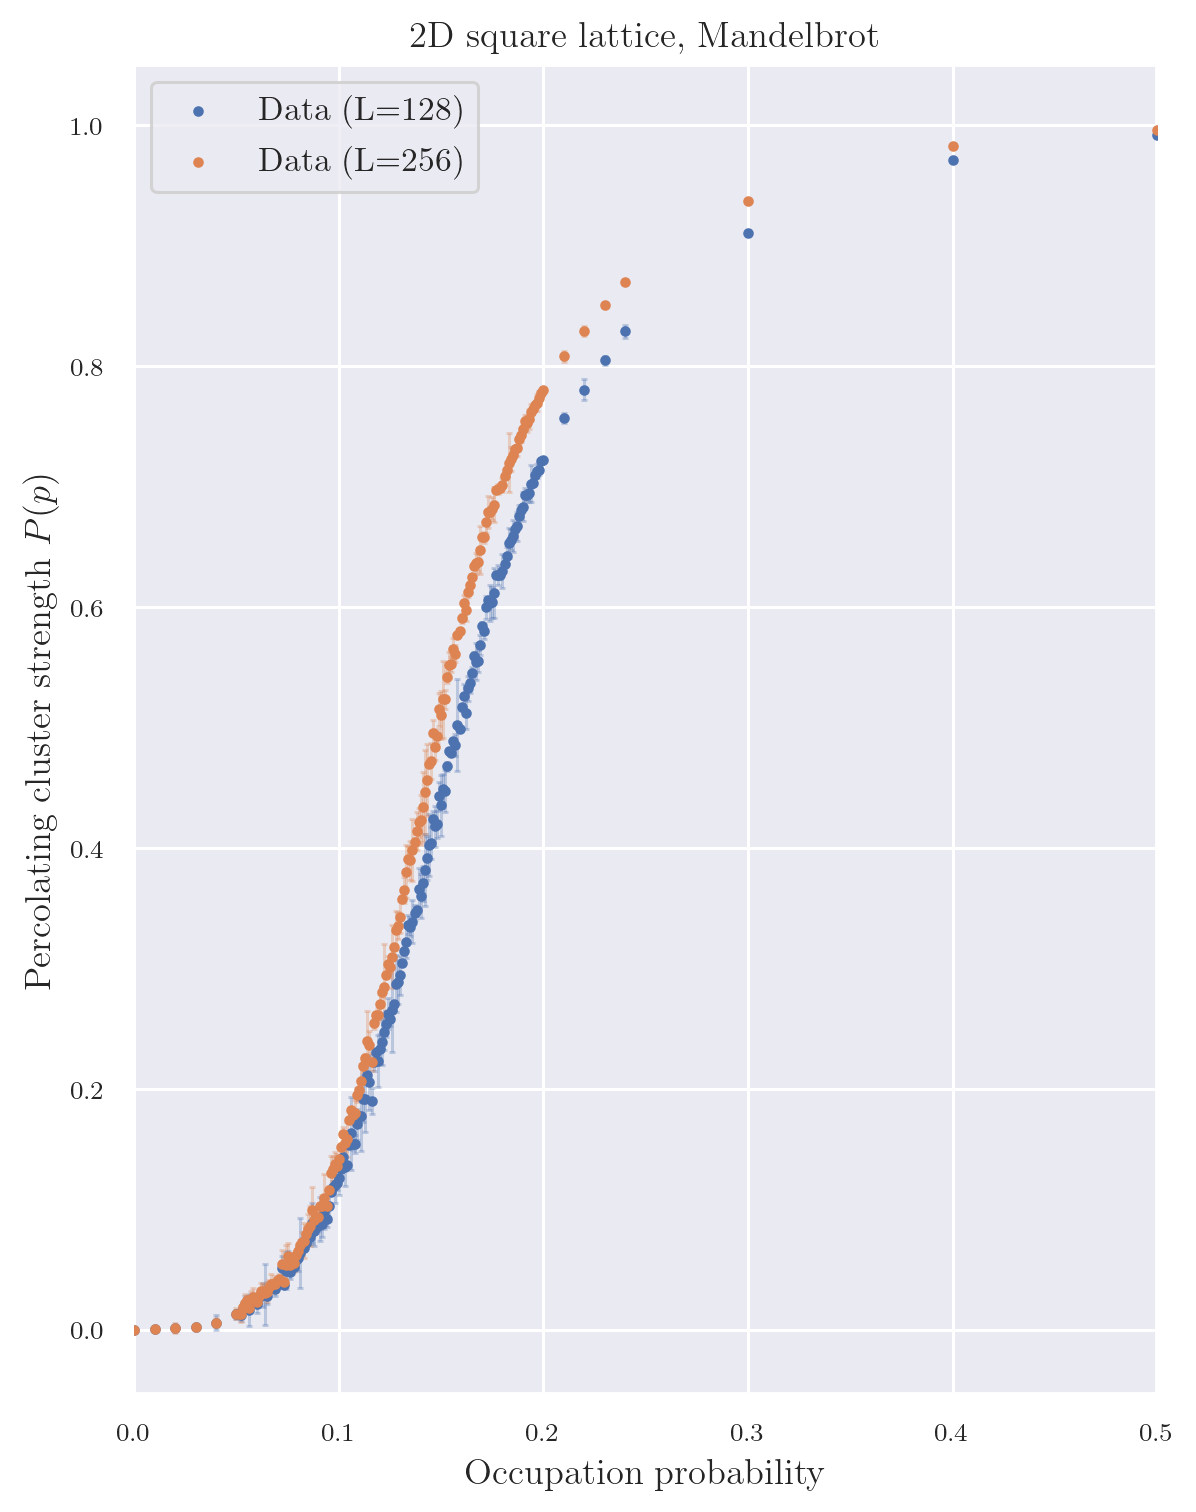
\includegraphics[width=\linewidth]{Images/simm_perc_clust_strength_1.png}
  \caption{Percolating cluster strength for the Mandelbrot percolation model}
  \label{fig:simm_perc_clust_strength_1}
\end{figure}

Other than the lower values for the critical occupation probability discussed above, another interesting fact worth pointing out is that although for both models the curve becomes essentially a linear function towards higher values of the occupation probability $p$, the slope of the curve is noticeably smaller for the Mandelbrot case. The reason for this is not immediately obvious and warrants further investigation.
The errors were computed using the same method as described in \autoref{sec:sim_perc_clust_strength}.


\section{Mean cluster size}

The results for the mean cluster size can be seen in \autoref{fig:simm_mean_cluster_size_1}. 

\begin{figure}[H]
  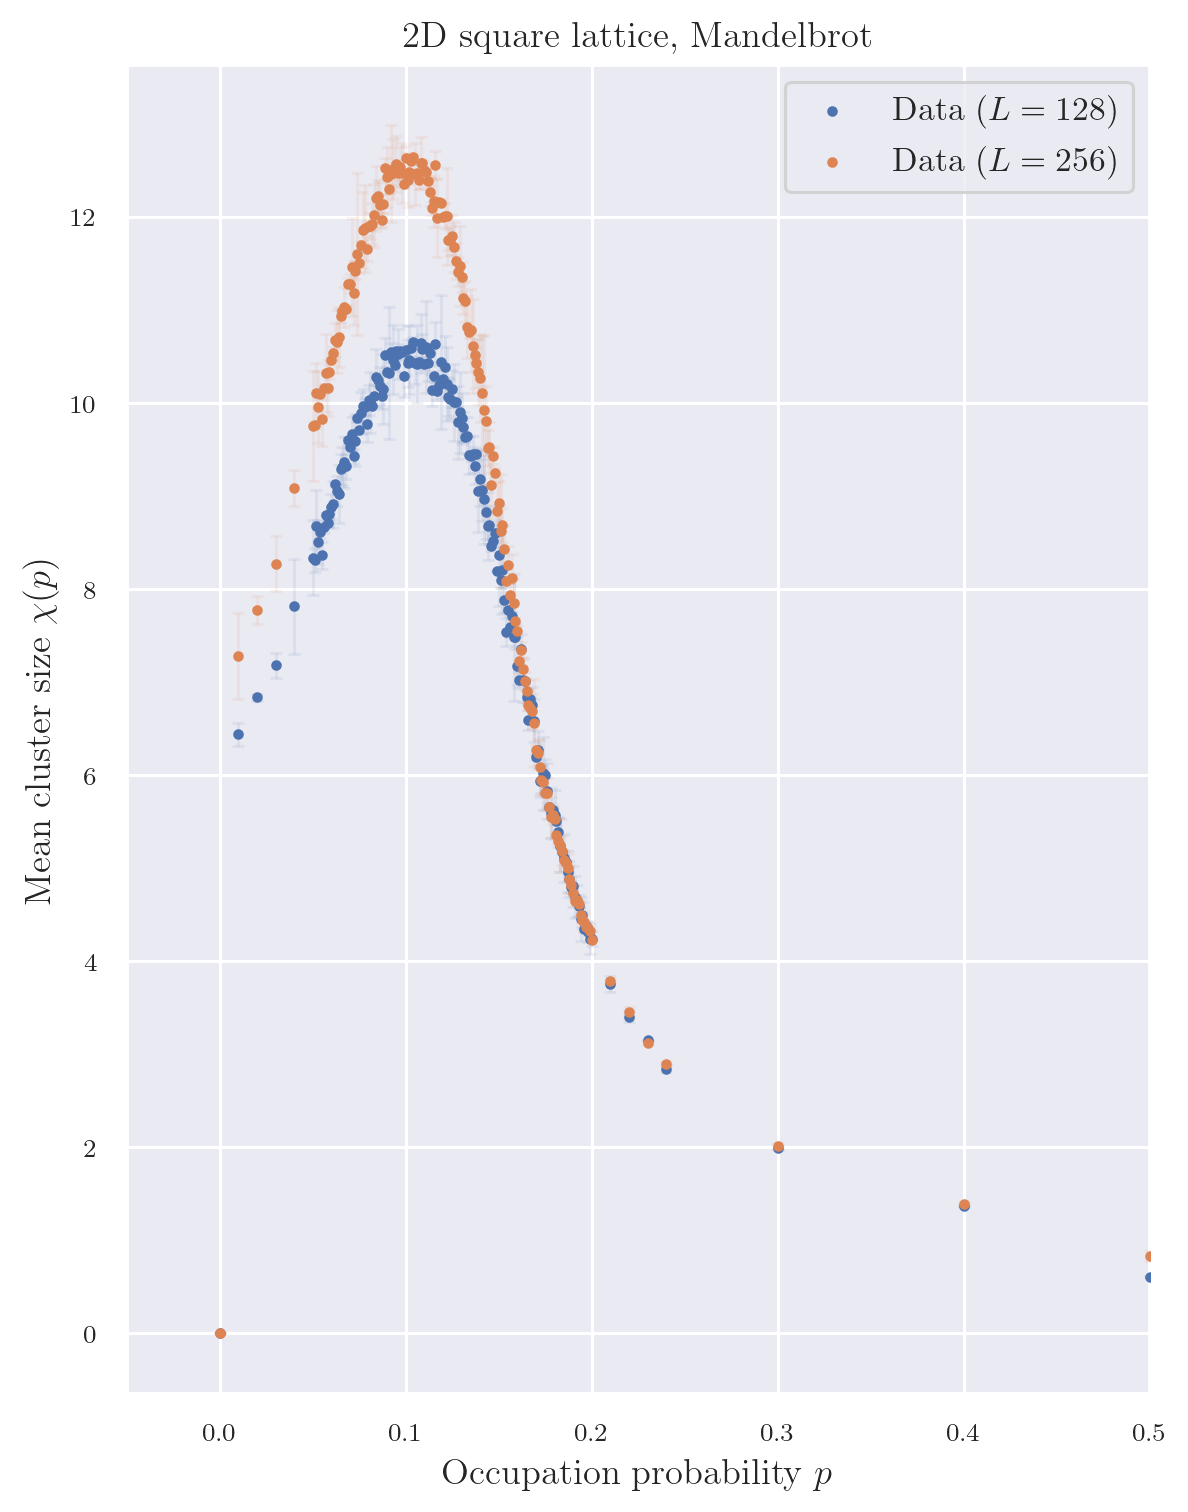
\includegraphics[width=\linewidth]{Images/simm_mean_cluster_size_1.png}
  \caption{Mean cluster size in the Mandelbrot percolation model}
  \label{fig:simm_mean_cluster_size_1}
\end{figure}

In comparison with the classical percolation plots (see \autoref{fig:sim_mean_cluster_size_1}), it is curious that the peak heights are smaller for the Mandelbrot percolation. The reason for this is, again not immediately obvious - the reader is invited to investigate this further.
The errors were computed using the same method as described in \autoref{sec:sim_mean_clust_size}.

\section{Conclusion}

Even in the case of classical percolation, which has been widely studied by many people in the last 50 years, we hope that this work provides a solid numerical and computation basis upon which further investigation can be made. We provide both the data used in these analysis and the code used to generate it in hopes of facilitating collaboration and reuse, as well as inspiring a more modern approach to computational research in general. 

For the case of Mandelbrot percolation, this work is intended as a first step towards computational analysis of the model, in particular emphasizing differences and similarities as compared to the classical percolation models. While we didn't intend to provide a through and careful theoretical justification of the results obtained, this is encouraged for the curious reader. 

The author is happy to answer any questions - feel free to email \url{alansammarone@gmail.com}.
 

% \cleardoublepage % Empty page before the start of the next part

%------------------------------------------------

% \part{Mandelbrot percolation} % Second part of the thesis

% \chapter{Mandelbrot percolation - methods and results}
\label{ch:mandelbrot_experimental}

\section{Introduction}

Now we turn our attention to the so called Mandelbrot percolation, which is also known in the literature as Fractal percolation. The idea is, again, to study the clusters structure and distribution, but the coloring of the lattice happens in a different way: instead of doing a single pass over the lattice and coloring the nodes at random, we do this process repeatedly - at each step, we subdivide each node in the lattice into a number of "sub-nodes" and color the remaining "alive" (not yet colored) nodes with probability $p$. An illustration of this process can be seen in \autoref{fig:mandelbrot_process}. 
Each iteration generates a lattice $A_n$ (which is, of course, highly correlated with the previous lattice $A_{n-1}$). Mandelbrot percolation is the study of the limit of this process the number of steps increases arbitrarily, that, is $\lim_{n\to\infty} A_n$.

\begin{figure}[H]
  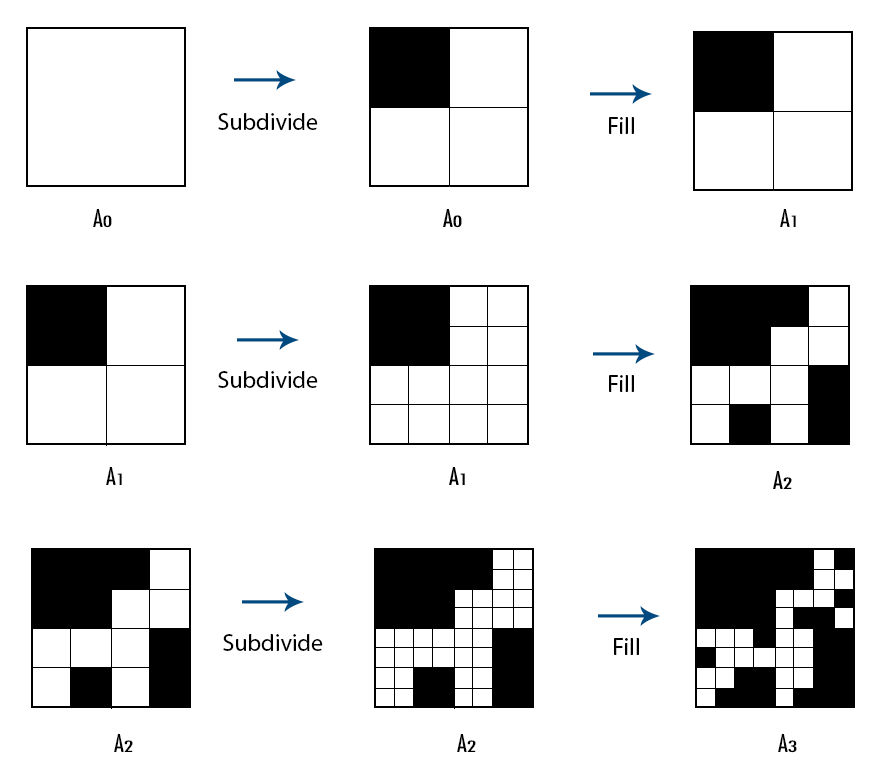
\includegraphics[width=\linewidth]{Images/mandelbrot_process.png}
  \caption{Illustration of the Mandelbrot percolation iteration process, showing three iterations}
  \label{fig:mandelbrot_process}
\end{figure}


\begin{figure}[H]
  \includegraphics[width=\linewidth]{Images/mandelbrot_lattice.png}
  \caption{A Mandelbrot percolation lattice after 11 iterations}
  \label{fig:mandelbrot_lattice}
\end{figure}


\section{Simulation methods}

The simulations were run, again, on a 2D periodic square lattice. 
We studied three properties: the percolation probability, mean cluster size and percolating cluster strength. We explicitly used exactly the same definitions, methods and algorithms as for the 2D case - the reason for this is that this way, a direct comparison is possible. The precise description of these methods is available in \autoref{ch:classical_experimental}.

\section{Percolation probability}

In \autoref{fig:simm_perc_prob_2}, the first thing we notice is that the the critical probability $p_c$ is much lower than in the classical percolation model - at first sight, it's clear that $p_c < 0.3$. The reason for this is somewhat obvious. For a given $(p, L)$ pair, in classical percolation, we do a single pass over the lattice, whereas in the Mandelbrot model, we have done several passes previously, when the lattice was smaller. So on top of making multiple passes, the previous passes happened when each node represented a bigger part fraction of the lattice.

\begin{figure}[H]
  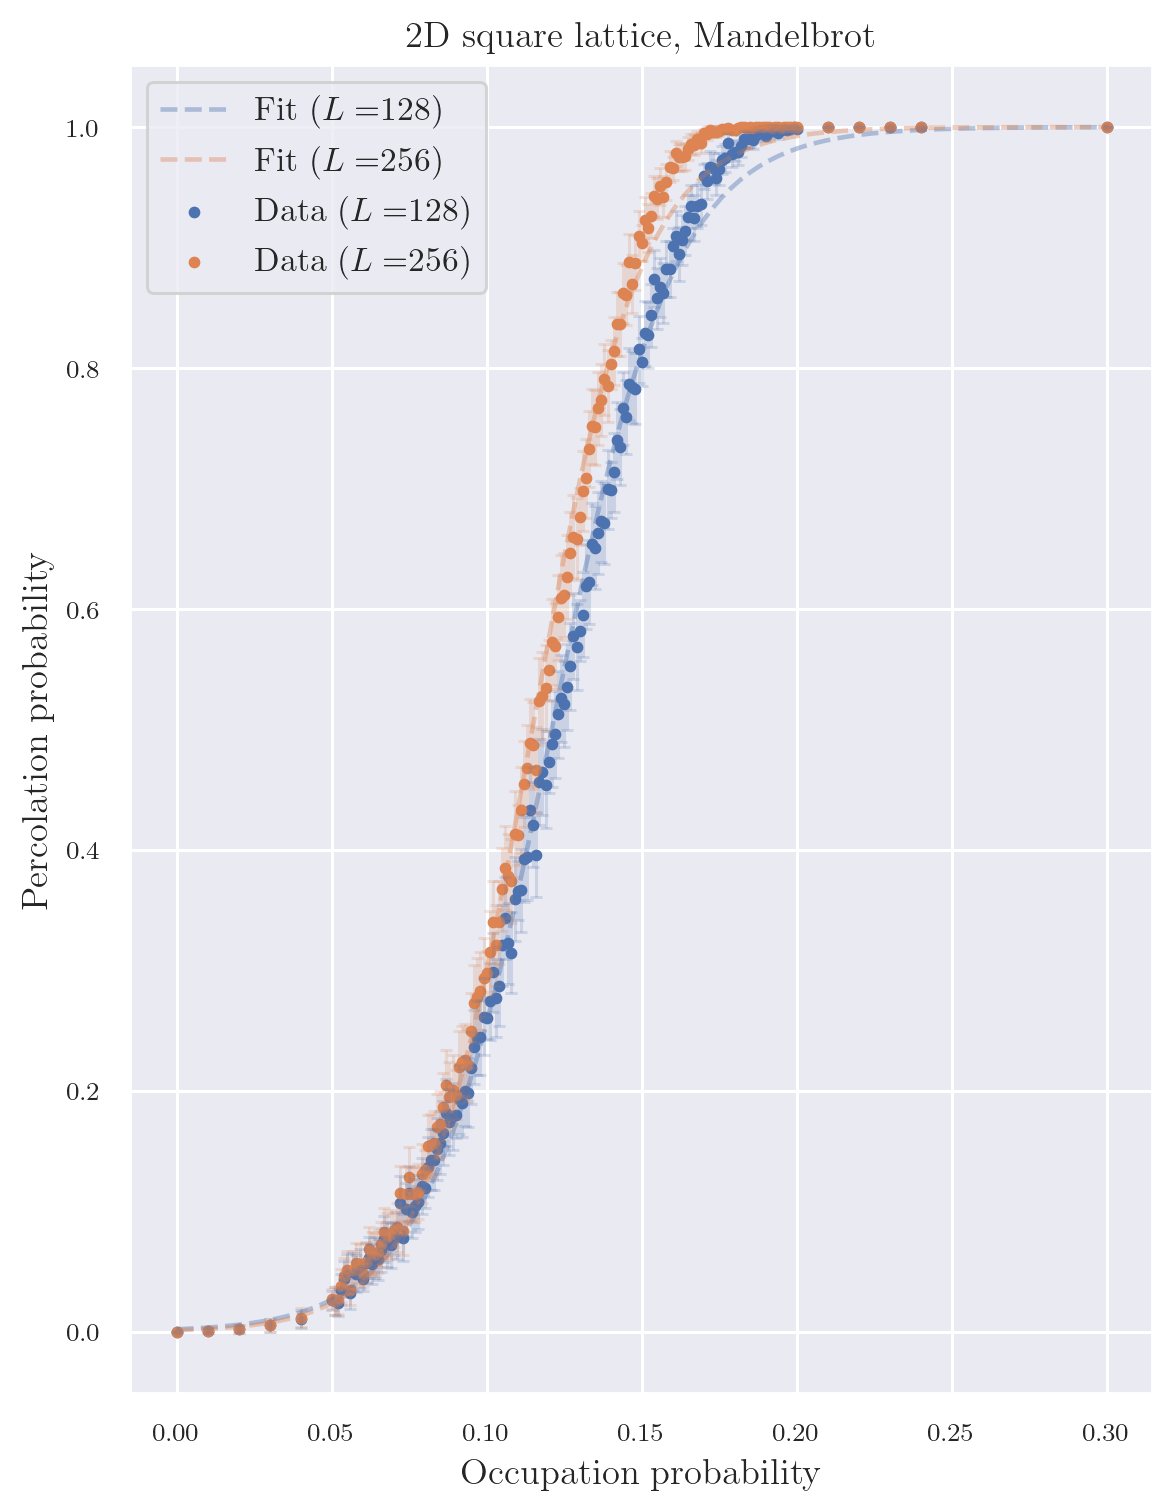
\includegraphics[width=\linewidth]{Images/simm_perc_prob_2.png}
  \caption{Percolation probability in the Mandelbrot percolation model}
  \label{fig:simm_perc_prob_2}
\end{figure}

Just like in classical percolation, we fitted a hyperbolic tangent function to the data, and for $L=256$, which is the largest size we simulated for the Mandelbrot model, we find that the the percolation probability reaches the $0.5$ mark when $p=\textbf{0.1273} \pm 0.021$. We point out that the fit is noticeably worse for the Mandelbrot model than in the case of classical percolation, which suggests an underlying fundamental difference between the models. Additionally, we notice that plots obtained for $L=128$ and $L=256$ are in relation to each other in a different way than the equivalent curves in the classical percolation case. In comparison with \autoref{fig:sim_perc_prob_2}, for example, one notices that whereas there, the curves have a sharp increase at very different occupation probabilities, here they are much closer to each other for low values of $p$, and remain much closer. We hypothesize that this happens, again, because the lattices are much more closely related here - the additional pass used in the $L=256$ happens at a smaller length scale and therefore has a less pronounced effect on the curve.

The errors were computed using the same method as described in \autoref{sec:sim_perc_prob}.

\section{Percolating cluster strength}

The percolation cluster strength results for the Mandelbrot percolation simulations can be seen in \autoref{fig:simm_perc_clust_strength_1}. The curve looks qualitatively pretty similar to the one we had for classical percolation (see \autoref{fig:sim_perc_clust_strength_1}).


\begin{figure}[H]
  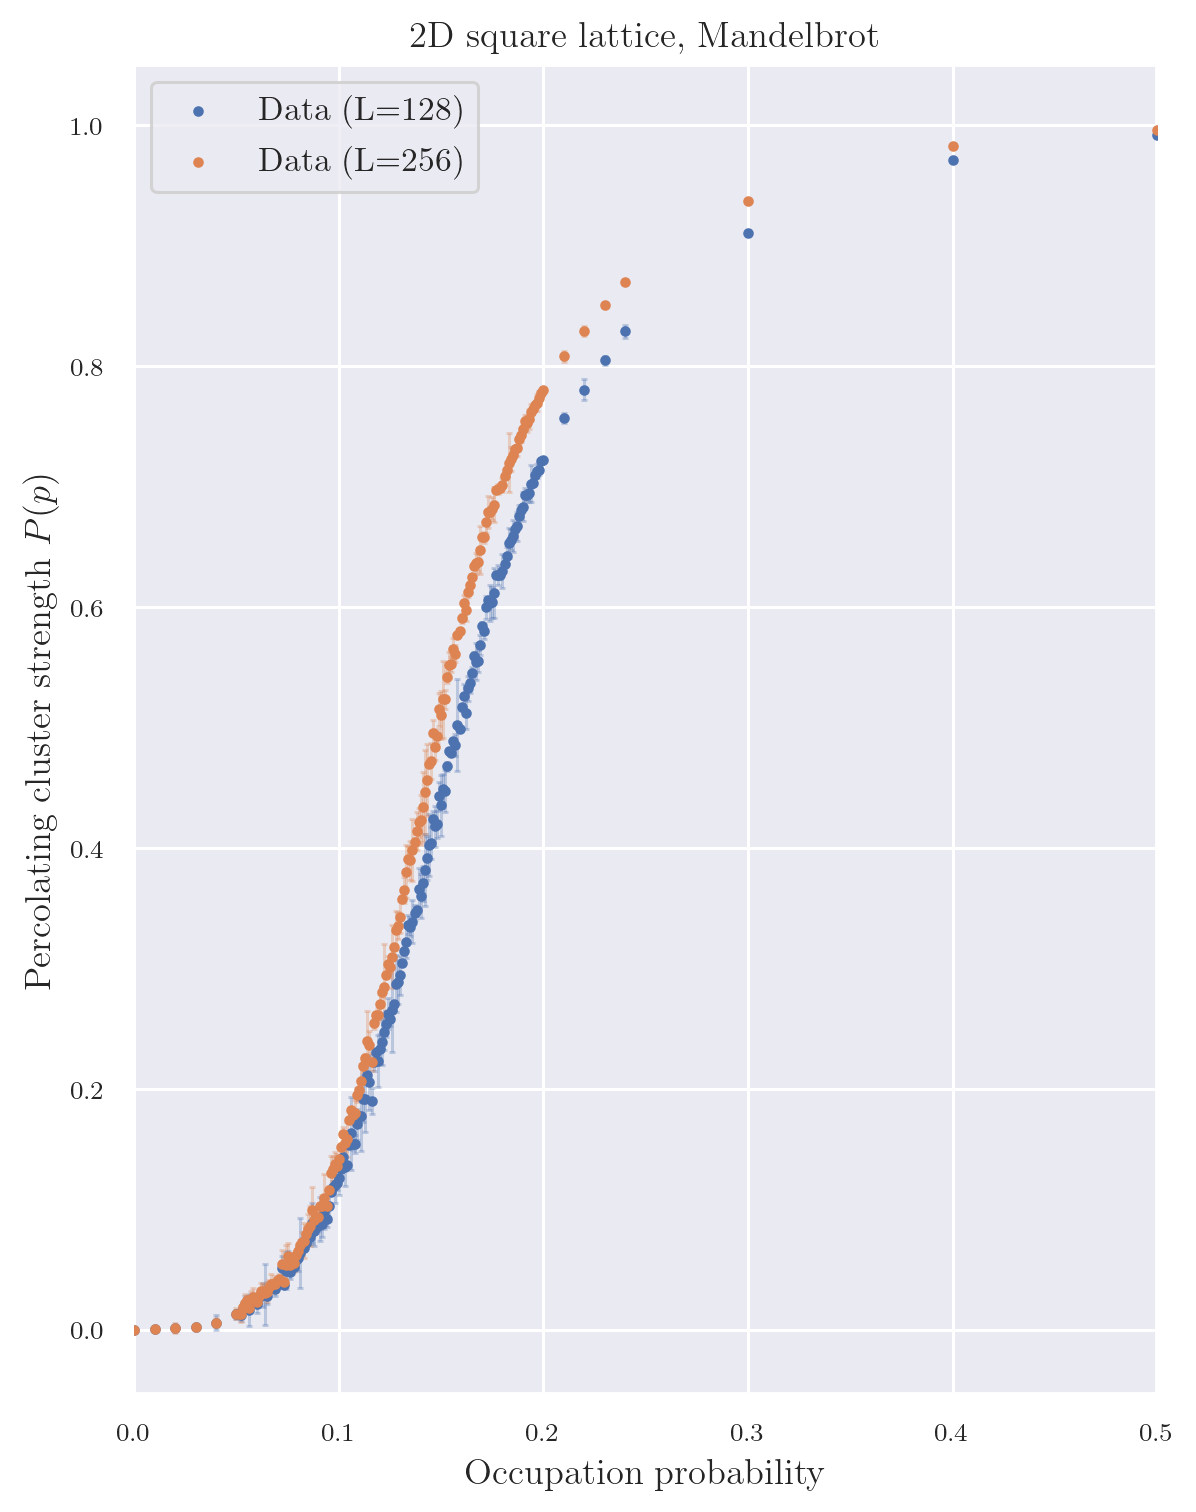
\includegraphics[width=\linewidth]{Images/simm_perc_clust_strength_1.png}
  \caption{Percolating cluster strength for the Mandelbrot percolation model}
  \label{fig:simm_perc_clust_strength_1}
\end{figure}

Other than the lower values for the critical occupation probability discussed above, another interesting fact worth pointing out is that although for both models the curve becomes essentially a linear function towards higher values of the occupation probability $p$, the slope of the curve is noticeably smaller for the Mandelbrot case. The reason for this is not immediately obvious and warrants further investigation.
The errors were computed using the same method as described in \autoref{sec:sim_perc_clust_strength}.


\section{Mean cluster size}

The results for the mean cluster size can be seen in \autoref{fig:simm_mean_cluster_size_1}. 

\begin{figure}[H]
  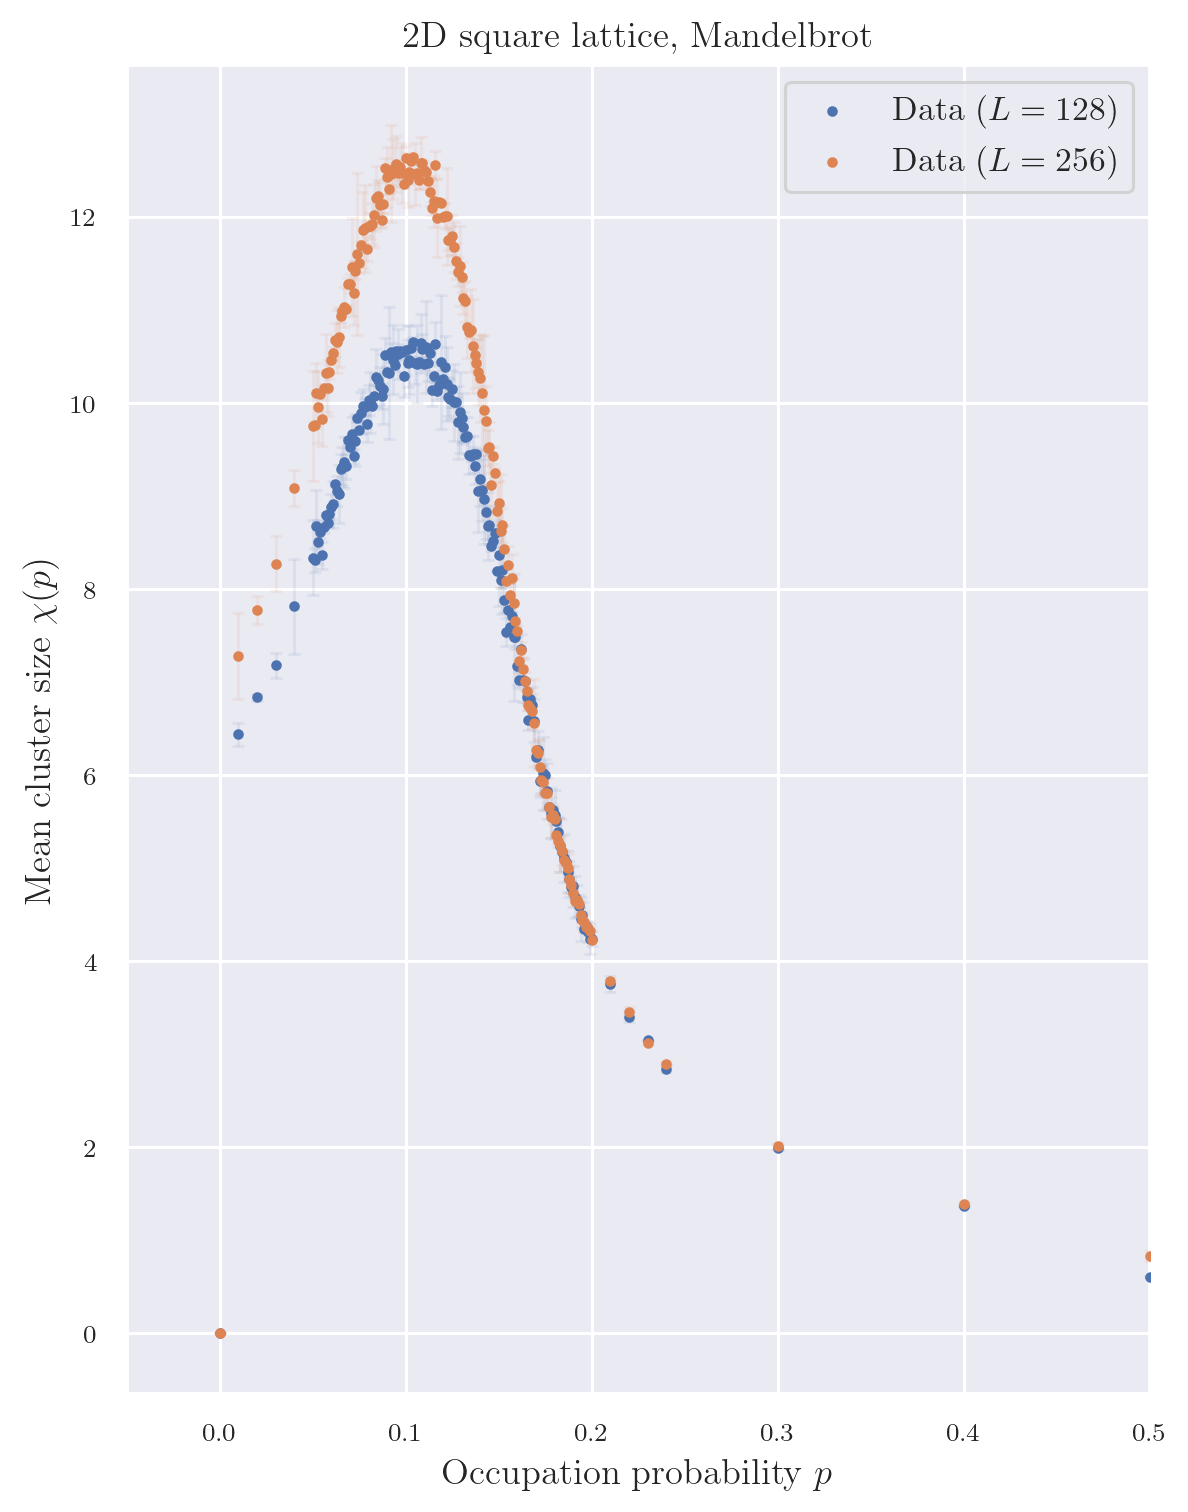
\includegraphics[width=\linewidth]{Images/simm_mean_cluster_size_1.png}
  \caption{Mean cluster size in the Mandelbrot percolation model}
  \label{fig:simm_mean_cluster_size_1}
\end{figure}

In comparison with the classical percolation plots (see \autoref{fig:sim_mean_cluster_size_1}), it is curious that the peak heights are smaller for the Mandelbrot percolation. The reason for this is, again not immediately obvious - the reader is invited to investigate this further.
The errors were computed using the same method as described in \autoref{sec:sim_mean_clust_size}.

\section{Conclusion}

Even in the case of classical percolation, which has been widely studied by many people in the last 50 years, we hope that this work provides a solid numerical and computation basis upon which further investigation can be made. We provide both the data used in these analysis and the code used to generate it in hopes of facilitating collaboration and reuse, as well as inspiring a more modern approach to computational research in general. 

For the case of Mandelbrot percolation, this work is intended as a first step towards computational analysis of the model, in particular emphasizing differences and similarities as compared to the classical percolation models. While we didn't intend to provide a through and careful theoretical justification of the results obtained, this is encouraged for the curious reader. 

The author is happy to answer any questions - feel free to email \url{alansammarone@gmail.com}.
 % Chapter 2

\afterpage{\blankpage} % Empty page before the start of the next part
%----------------------------------------------------------------------------------------
%	POST-CONTENT THESIS PAGES
%----------------------------------------------------------------------------------------
\clearpage
% \appendixpage
% \addappheadtotoc
\part{Appendix}
\appendix
\chapter{Code}
\label{chap:code}


\section{Overview}
Musk is a Python library developed as part of this work to help us run and store simulations and statistics in a distributed, highly parallel fashion. The code is available in Github\footnote{\url{https://github.com/alansammarone/musk}}.

To achieve an arbitrary amount of parallelism, Musk makes use of an independent queue service. The current version uses Amazon SQS\footnote{\url{https://aws.amazon.com/sqs/}}, but the code is easily extensible to make use of other popular queue services, such as RabbitMQ or Kafka. The general idea is that there a script (referred to as the enqueuer) which sends messages to a specific queue, and each message represents a particular computation one wishes to perform. This is what a message looks like (in terms of data structures, it is just a Python dictionary):

\begin{python}
{
    "parameters": {
        "probability": 0.553, 
        "size":256,
        "repeat":128
    } 
}

\end{python}

This particular message encapsulates the parameters of the simulation we want to run - the occupation probability, the lattice size, and how many time we want to repeat the process. In general, one generates thousands of messages like this and sends them to a queue (which is particular to a specific type of model - 2D classical percolation and Mandelbrot percolation, for example, have different queues), where they sit and wait further processing. We also have messages that represent instructions to compute statistics for a particular simulation, such as mean cluster size and percolation probability, but they follow the same general structure.


We also have a script called the dequeuer. It can (and should, in general) run on a number of separate machine and it's job is to read from messages from a queue and process them. Since it is completely separate from the enqueuer, we can horizontally scale the system as much as like - during our simulations, we used up to 30 virtual machines running 2 instances of dequeuer each, for a total of 60 dequeuer processes constantly (once every 2 seconds) reading the queues and in case a message is found, processing it and then deleting it. 

To store data, we use the popular open source database called MySQL\footnote{\url{https://www.mysql.com/}}. Each simulation is stored as a row, containing the parameters as well as clusters on the lattice after the simulation is run. The statistics (mean cluster size, percolating cluster strength, etc) are stored as rows on a different table.


In general, the process to run the simulations and statistical analysis is the following:

\begin{enumerate}
  \item Run the simulation enqueuer with the appropriate parameter range configuration to generate messages representing the simulations one wishes to run
  \item Run the simulation dequeuer (potentially on multiple machines) and wait for all the computation to finish (depending on the number of messages, this could take weeks). This is generate many rows in the MySQL database.
  \item Run the statistics enqueuer, which will read the rows written in the previous step and generate one message per row 
  \item Run the statistics dequeuer, which will read the messages sent to the queue in the previous step, compute the desired statistics, and write the results in a separate table.
\end{enumerate}

\section{Classes and scripts}

The library is made up of several classes, each having a particular responsibility and implementation. We hope this section can serve as inspiration for anyone interested in using this library and/or coding their own distributed processing framework.

\begin{itemize}
    \raggedright\item \textbf{Lattice classes} (\pyth{Lattice}, \pyth{Square2DLattice}, \pyth{Square2DPeriodicLattice} and \pyth{Square2DFiniteLattice})\footnote{\url{https://github.com/alansammarone/musk/tree/master/musk/lattices}}: These represent the lattices, in increasing order of specialization (via inheritance). They contain operations such as neighbour resolution, filling the lattice randomly, subdividing, and cluster computations.
    
    \raggedright\item \textbf{Model classes} (\pyth{PercolationModel}, \pyth{PercolationStatsModel}, \pyth{P2MModel} and \pyth{P2MStatsModel})\footnote{\url{https://github.com/alansammarone/musk/tree/master/musk/percolation}}: Models contain the interface to the database - each model class represents a single database table, and contains one attribute for each column in the corresponding table. The class also contain SQL queries for reading/writing. An instance of this class represents a row.
    
    \raggedright\item \textbf{Simulation classes} (\pyth{Simulation}, \pyth{PercolationSimulation} and \pyth{P2MSimulation})\footnote{\url{https://github.com/alansammarone/musk/tree/master/musk/percolation}}: Simulation classes use the lattice classes to actually execute the simulations, and then use the model classes to store and/or retrieve the results to/from the database.
    
    
    \raggedright\item \textbf{Processor classes} (\pyth{Processor}, \pyth{PercolationProcessor} and \pyth{PercolationStatsProcessor}, \pyth{PercolationStatsProcessor}, \pyth{P2MProcessor})\footnote{\url{https://github.com/alansammarone/musk/tree/master/musk/percolation}}: Processors are responsible for processing a queue message (and then, if the processing was successful, deleting the message). In the case of simulations, they delegate the bulk of the work to the \pyth{Simulation} classes described above. In the case of statistics, they contain the statistics computations directly.
    
    \raggedright\item \textbf{Queue-related classes} (\pyth{Queue}, \pyth{Message}, \pyth{SQSQueue},  \pyth{SQSMessage})\footnote{\url{https://github.com/alansammarone/musk/tree/master/musk/core}}: These are responsible for various aspects of the queue system - creating and updating queues, as well as sending, reading and deleting messages from them.
    
    \raggedright\item \textbf{Dequeuer class} (\pyth{Dequeuer})\footnote{\url{https://github.com/alansammarone/musk/blob/master/musk/core/dequeuer.py}}: This class receives an instance of the \pyth{Queue} class and an instance of a \pyth{Processor} class. Is is then responsible for reading messages from the queue and appropriately routing them to the processor instance. 
    
    
    \raggedright\item\textbf{Dequeuer runner class and script} (\pyth{DequeuerRunner})\footnote{\url{https://github.com/alansammarone/musk/blob/master/scripts/dequeuer_runner.py}}: The \pyth{DequeuerRunner} class collects a set of dequeuer instances (one for each queue-processor pair) and is responsible for scheduling the execution of each. This includes spawning  new processes to handle messages after a given threshold is reached (this is necessary since Python contains inherent memory leaks that are very hard to deal with - it's simpler to just rerun the interpreter in a new process). There is also a \pyth{run_dequeuer.sh} script which is responsible for actually running the main Python file with correct environment variables and permissions.
    
    \raggedright\item \textbf{Enqueuer script} \footnote{\url{https://github.com/alansammarone/musk/blob/master/scripts/enqueuer.py}}: This script is responsible for generating and sending messages to their appropriate queue for actual processing (which is done by the dequeuer classes described above).
    
    
\section{Deployment}

Musk can be deployed quickly to any number of worker nodes (the deploy happens in parallel, so deploying to 100 workers takes around the same time as deploying to a single worker), each of which will process messages and write to the database independently of the others. To accomplish this, we use Ansible\footnote{\url{https://www.ansible.com}}, an open source automation tool supported by the Red Hat foundation. After configuring the inventory file, one simply needs to run the playbook filefile\footnote{\url{https://github.com/alansammarone/musk/blob/master/deploy/worker.yaml}} (using \pyth{ansible-playbook}), which will then, in all worker nodes, install the proper version of Python, all the required dependencies, set up configuration files, clone the Github repository, and set up a cron job to watch the queues (which is run every minute, but this can easily be changed in the configurations).

\end{itemize}

\clearpage

\chapter{Data}
\label{chap:data}
We provide the simulation data used in this work as a \pyth{.sql} file\footnote{\url{http://tiny.cc/muskdatadump}}, which is a MySQL database dump. If this file is not available at the time of reading, simply contact the author at the email address provided at the beginning of the thesis.


Below, for every table, we describe the fields and their data types. Each row corresponds to a particular simulation sample. The tables contains several dozen million rows each.

\begin{itemize}
    \item Table \textbf{p2s}: This table contains the simulation data for the classical 2D square percolation model
    \begin{itemize}
        \item \textbf{id} int: A primary key which uniquely identifies each row
        \item \textbf{probability} float: The occupation probability used in this simulation
        \item \textbf{size} smallint: The size of the lattice - note that a 2D square lattice with a given size has $\textrm{size}^2$ nodes.
        \item \textbf{observables} mediumblob: Contains a bz2-compressed list of clusters present in the lattice
        \item \textbf{took} float: How long the simulation took
        \item \textbf{created} timestamp: The time at which this simulation was created.
    \end{itemize}
    \item Table \textbf{p2s\_stats}: This table contains the statistics for every simulation in the \textbf{p2s} table. There is a one-to-one relation between every row in both tables (this is encoded in the \textbf{simulation\_id} column described below).
    \begin{itemize}
        \item \textbf{id} int: A primary key which uniquely identifies each row
        \item \textbf{simulation\_id} int: A foreign key pointing to the equivalent row in the \textbf{p2s} table from which these statistics were computed.
        \item \textbf{probability} float: The occupation probability of the simulation associated with this row
        \item \textbf{size} smallint: The size of the lattice used in the simulation associated with this row
        \item \textbf{has\_percolate d} tinyint: Whether the associated lattice has percolated
        \item \textbf{cluster\_size\_histogram} text: A histogram of the cluster sizes in the associated lattice
        \item \textbf{mean\_cluster\_size} float: Average size of the clusters in the associated lattice
        \item \textbf{correlation\_function} longtext: Correlation function approximation in the associated lattice
        \item \textbf{percolating\_cluster\_strength} float: Percolating cluster strength in the associated lattice (0 if the lattice has not percolated).
    \end{itemize}    
    \item Table \textbf{p2m}: Exactly the same structure as the \textbf{p2s} table, but each row contains simulation data for a 2D Mandelbrot simulation.
    \item Table \textbf{p2m\_stats}: Exactly the same structure as the \textbf{p2s\_stats} table, but contains the statistics for the Mandelbrot simulations stored in the \textbf{p2m} table.
    
\end{itemize}

\clearpage
\clearpage
\chapter{Tables}
\begin{table}[H]
\begin{center}
    \begin{tabular}{||c | c |  c|| }
    \hline
      Size &   $\alpha$ &   $\beta$ \\
    \hline
      16 &    17.316  &  0.502909 \\
      24 &    22.9593 &  0.523217 \\
      32 &    28.7445 &  0.535866 \\
      48 &    37.8221 &  0.549603 \\
      64 &    46.2392 &  0.557582 \\
      96 &    61.2356 &  0.566495 \\
     128 &    75.4226 &  0.571311 \\
     192 &   102.451  &  0.576883 \\
     256 &   126.736  &  0.579948 \\
     294 &   139.832  &  0.581133 \\
    \hline
    \end{tabular}
\end{center}
\caption{Hyperbolic tangent least squares fit parameters}
\label{table:sec3_tahn_fit_parameters}
\end{table}



\begin{table}[H]
\begin{center}
    \begin{tabular}{||c |c| c|| }
    \hline
      Parameter &  value & standard deviation \\
    \hline
      $a$ &    1.56  &  0.08 \\
      $b$ &    4.3 &  0.83 \\
      $n$ & 0.786 & 0.0088 \\
    \hline
    \end{tabular}
\end{center}
\caption{Percolation probability, $\alpha$ finite-size scaling parameters}
\label{table:pp_slope_finite_size_scaling_params}
\end{table}


\begin{table}[H]
\begin{center}
    \begin{tabular}{||c | c c|| }
    \hline
      Parameter &  value & standard deviation \\
    \hline
      $a$ &    38.2  &  44.12 \\
      $b$ &    0.22 &  0.053 \\
      $c$ & 0.590 & 0.00074 \\
      $n$ & 0.10 & 0.02 \\
    \hline
    \end{tabular}
\end{center}
\caption{Percolation probability, $\beta$ finite-size scaling parameters}
\label{table:pp_center_finite_size_scaling_params}
\end{table}






\begin{table}[H]
\begin{center}
    \begin{tabular}{||c | c|| }
    \hline
       Size & Peak height     \\
    \hline
         16 & 5.31 $\pm$ 0.162  \\
         24 & 6.75 $\pm$ 0.135  \\
         32 & 7.93 $\pm$ 0.203  \\
         48 & 9.5 $\pm$ 0.197   \\
         64 & 10.76 $\pm$ 0.249 \\
         96 & 12.48 $\pm$ 0.283 \\
        128 & 13.51 $\pm$ 0.272 \\
        192 & 14.96 $\pm$ 0.294 \\
        256 & 15.86 $\pm$ 0.298 \\
        294 & 16.27 $\pm$ 0.302 \\
        512 & 17.78 $\pm$ 0.392 \\
    \hline
    \end{tabular}
\end{center}
\caption{Mean cluster size, peak height}
\label{table:pp_mean_cluster_size_peak_values}
\end{table}



\begin{table}[H]
\begin{center}
    \begin{tabular}{||c | c|| }
    \hline
       Size & Peak height     \\
    \hline
         24 & 0.52 $\pm$ 0.032  \\
         32 & 0.53 $\pm$ 0.053  \\
         48 & 0.54 $\pm$ 0.01   \\
         64 & 0.552 $\pm$ 0.051 \\
         96 & 0.557 $\pm$ 0.044 \\
        128 & 0.562 $\pm$ 0.025 \\
        192 & 0.569 $\pm$ 0.03  \\
        256 & 0.575 $\pm$ 0.049 \\
        294 & 0.576 $\pm$ 0.024 \\
        512 & 0.581 $\pm$ 0.02  \\
    \hline
    \end{tabular}
\end{center}
\caption{Mean cluster size, peak positions}
\label{table:pp_mean_cluster_size_peak_positions}
\end{table}


\begin{table}[H]
\begin{center}
    \begin{tabular}{||c | c c|| }
    \hline
      Parameter &  value & standard deviation \\
    \hline
      $a$ &    2.02558273e+03  &  3.19001498e+06 \\
      $b$ &    1.58092558e+02 &  9.87273040e+03 \\
      $c$ & 8.59573639e-03 & 6.62713676e+00  \\
      $n$ & -4.09236591e+03 & 3.19134574e+06 \\
    \hline
    \end{tabular}
\end{center}
\caption{Mean cluster size, peak position finite-size scaling parameters}
\label{table:pp_mean_cluster_size_peak_height_finite_size_scaling_params}
\end{table}


\begin{table}[H]
\begin{center}
    \begin{tabular}{||c | c c|| }
    \hline
      Parameter &  value & standard deviation \\
    \hline
      $a$ &    275.7  &  31.85 \\
      $b$ &    0.146 &  0.93 \\
      $c$ & 0.5986 & 0.0040 \\
      $n$ & 0.5566 & 0.05 \\
    \hline
    \end{tabular}
\end{center}
\caption{Mean cluster size, peak position finite-size scaling parameters}
\label{table:pp_mean_cluster_size_peak_position_finite_size_scaling_params}
\end{table}


 


\cleardoublepage%********************************************************************
% Bibliography
%*******************************************************
% work-around to have small caps also here in the headline
% https://tex.stackexchange.com/questions/188126/wrong-header-in-bibliography-classicthesis
% Thanks to Enrico Gregorio
\defbibheading{bibintoc}[\bibname]{%
  \phantomsection
  \manualmark
  \markboth{\spacedlowsmallcaps{#1}}{\spacedlowsmallcaps{#1}}%
  \addtocontents{toc}{\protect\vspace{\beforebibskip}}%
  \addcontentsline{toc}{chapter}{\tocEntry{#1}}%
  \chapter*{#1}%
}
\nocite{*}
\printbibliography[heading=bibintoc]
 % Bibliography

%----------------------------------------------------------------------------------------

\end{document}
